% !TeX root = ./maltoni_niccolo_tesi.tex
% !TeX encoding = UTF-8 Unicode
% !TeX spellcheck = it_IT
% !TeX program = arara
% !TeX options = --log --verbose --language=it "%DOC%"

% arara: lualatex:      { interaction: batchmode, shell: yes }
% arara: frontespizio:  { interaction: batchmode, engine: lualatex, shell: yes }
% arara: biber
% arara: lualatex:      { interaction: batchmode, shell: yes }
% arara: lualatex:      { interaction: nonstopmode, shell: yes, synctex: yes }

\documentclass[%
  a4paper,                % formato di pagina A4
  fontsize=12pt,          % corpo del testo a 12pt
  % la dimensione 12pt automaticamente imposta \footnotesize a 10pt
  oneside,                % TODO: change (oneside|twoside) documento a singola o doppia facciata,
  openany,              % (openany|openright) fa cominciare un capitolo nella successiva pagina a disposizione o sempre in una pagina destra
  % twocolumn,            % dà a LaTeX le istruzioni per comporre l'intero documento su due colonne
  titlepage,              % (titlepage|notitlepage) se dopo il titolo del documento debbaavere  inizio  una  nuova  pagina
  % fleqn,                % allinea le formule a sinistra rispetto a un margine rientrato
  % leqno,                % mette la numerazione delle formule a sinistra anziché a destra
  final                   % (draft|final) scelta tra bozza o finale, influenza il comportamento degli altri pacchetti
  headings=standardclasses, % changes the font of all section heading levels to serif
  headings=big,             % revert to default heading size that headings=standardclasses changes
  chapterprefix=false       % reverse the chapterprefix=true option that headings=standardclasses sets
]{scrbook}

\usepackage{fancyvrb}       % fornisce l'ambiente VerbatimOut e modifica listati di codice

\begin{VerbatimOut}{\jobname.xmpdata}
\Title{Progettazione di una piattaforma web per la simulazione di programmi aggregati}
\Author{Niccolò Maltoni}
\Keywords{Aggregate programming\sep{}Protelis\sep{}Applicazione web\sep{}Simulazione}
\Copyright{Questo documento è fornito sotto licenza Creative Commons Attribution-ShareAlike 4.0 International}
\CopyrightURL{http://creativecommons.org/licenses/by-sa/4.0}
\end{VerbatimOut}

\def\blx@nowarnpolyglossia{}
\usepackage{unibotesi}

\usepackage[automark,headsepline]{scrlayer-scrpage}
\clearpairofpagestyles{}
\cfoot[\pagemark]{\pagemark}
\lehead{\headmark}
\rohead{\headmark}
\pagestyle{scrheadings}

\usepackage{lipsum}

\begin{document}

  \frontmatter{}

  \begin{Preambolo*}
  \usepackage{fontspec}
  \defaultfontfeatures{ Scale = MatchUppercase }
  \setmainfont{libertinusserif}[
    Scale=1.0,
    Ligatures={Common, TeX},
    % Numbers={OldStyle, Proportional},
    UprightFont={*-regular},
    BoldFont={*-bold},
    ItalicFont={*-italic},
    BoldItalicFont={*-bolditalic},
    Extension=.otf
  ]
  \setsansfont{libertinussans}[
    Ligatures={Common, TeX},
    % Numbers={OldStyle, Proportional},
    UprightFont={*-regular},
    BoldFont={*-bold},
    ItalicFont={*-italic},
    % BoldItalicFont={*-bolditalic},
    Extension=.otf
  ]
  \setmonofont{libertinusmono}[
    Scale=0.95,
    UprightFont={*-regular},
    % BoldFont={*-bold},
    % ItalicFont={*-italic},
    % BoldItalicFont={*-bolditalic},
    Extension=.otf
  ]
\end{Preambolo*}
\begin{frontespizio}
  \Universita{Bologna}        % aggiunge da sé “Università degli Studi di”.
  \Istituzione{%
    Alma Mater Studiorum --- Università di Bologna \\%
    Campus di Cesena%
  }
  \Divisione{Dipartimento di Informatica --- Scienza e Ingegneria}
  \Corso[Laurea magistrale]{Ingegneria e Scienze Informatiche}
  \Annoaccademico{2019--2020}
  \Titolo{Progettazione di una piattaforma web\\per la simulazione di programmi aggregati}
  \Sottotitolo{Tesi in Pervasive Computing}
  % \Preambolo{\renewcommand{\frontsmallfont}[1]{\small}}       % non viene stampata la matricola
  % \Preambolo{\renewcommand{\frontsmallfont}[1]{\small Matr.}} % abbrevia la matricola
  \Candidato[840825]{Niccolò~Maltoni}
  \NCandidato{Presentata da}  % sostituisce la parola “Candidato”
  \Relatore{Prof.~Mirko~Viroli}
  \Correlatore{Prof.~Danilo~Pianini}
  \Piede{%                    % sostituisce la scritta “Anno Accademico” nel piede
    III sessione di laurea \\%
    Anno Accademico 2019--2020%
  }
\end{frontespizio}

% Necessario per Overleaf: compila il TeX del frontespizio subito dopo averlo generato
\IfFileExists{\jobname-frn.pdf}{}{%
\immediate\write18{lualatex \jobname-frn}}

  \clearemptydoublepage{}
\thispagestyle{empty}
\vspace*{20ex}
\begin{flushright}
    \begin{LARGE}
        \textbf{Parole chiave}\\
        \vspace{5ex}
    \end{LARGE}
    \begin{normalsize}
      \textbf{%
        Aggregate computing\\%
        \medskip
        Aggregate programming\\%
        \medskip
        Protelis\\%
        \medskip
        Applicazione web\\%
        \medskip
        Simulazione
      }
    \end{normalsize}
\end{flushright}
\vfill

  \clearemptydoublepage{}
\thispagestyle{plain}
\null{}\vspace{\stretch{1}}
\begin{flushright}
  \textit{%
    A tutti gli amici e i familiari che mi hanno sostenuto.\\
    A chi non ha potuto assistere anche a questo mio traguardo.
  }
\end{flushright}
\vspace{\stretch{2}}\null{}

  \begin{abstract}
  % \strong{TODO}
  \todo[inline]{Il sommario verrà scritto per ultimo; di seguito un lorem ipsum per dare l'idea}
  \lipsum[1-2] % ChkTeX 8
\end{abstract}


  \tableofcontents

  \mainmatter{}

  \addchap{Introduzione}\label{ch:intro}

% Nel corso degli ultimi anni i sistemi informatici hanno avuto uno sviluppo sempre crescente,
Nel corso degli ultimi anni i sistemi informatici hanno avuto uno sviluppo notevole.
Grazie all'incremento della potenza computazionale disponibile a basso costo, alla riduzione delle dimensioni delle unità di calcolo e alla diffusione delle reti wireless,
ormai molti degli ambienti in cui vive la maggior parte della popolazione sono pervasi di sensori (il cosiddetto \emph{IoT}, Internet delle Cose) e di dispositivi ``smart'' (come smartphone e tablet).

Questo ha portato alla necessità di programmare sistemi distribuiti composti da numerosi dispositivi che devono potersi coordinare tra loro
per poter portare a termine la computazione.

La \emph{programmazione aggregata} è un approccio promettente per lo sviluppo di sistemi di questo tipo.
Tale paradigma è basato sull'impianto teorico del \emph{field calculus} e ha visto negli ultimi anni la realizzazione,
da parte dell'Università di Bologna, di linguaggi e framework innovativi per la sua applicazione in contesti d'uso reale:
\emph{Protelis} e \emph{ScaFi}.

Entrambi si avvalgono della piattaforma JVM (\emph{\emph{J}ava \emph{V}irtual \emph{M}achine}) per poter essere eseguiti;
come vedremo, questo garantisce numerose proprietà, ma può essere limitante in contesti didattici.
Infatti, la necessità di possedere una rete reale di dispositivi o di configurare un simulatore per l'esecuzione
aggiunge ulteriore complessità per un novizio che voglia approcciarsi alla tecnologia.
Inoltre, non è da ignorare nemmeno la necessità di configurazione di un progetto Gradle o SBT completo per poter realizzare un prototipo minimale.

In tempi recenti anche il web è maturato molto:
l'evoluzione tecnologica ha permesso di realizzare applicazioni utilizzabili tramite browser con livelli di complessità comparabili alle controparti desktop,
senza il carico aggiuntivo, dal punto di vista dell'utente, dell'installazione e della configurazione.
Inoltre, servizi complessi possono non dipendere esclusivamente dalle risorse computazionali dei dispositivi dell'utente,
bensì sfruttarle solo quando necessario, appoggiandosi alla potenza computazionale di un server di backend per le operazioni più complesse.

Si è dunque ritenuto utile realizzare un sistema web semplice e immediato da usare che permetta di abbozzare esempi di codice aggregato
(Protelis, nel prototipo implementato per questa tesi) e poterlo eseguire senza disporre di una rete di dispositivi o di un simulatore configurati per lo scopo.
In particolare, si è deciso di propendere per l'implementazione di un backend reattivo su piattaforma JVM che esegue il codice inviato dal client su una rete di dispositivi simulata tramite il simulatore Alchemist~\cite{alchemist-jos2013}.
Il client è una \emph{Single-Page Application} statica che permette lo sviluppo di codice direttamente dal browser e comunica con il server tramite un bus di eventi via socket.

\bigskip

Il documento è suddiviso in tre \nameCrefs{part:background} principali.

Nella~\Cref{part:background} viene fatta una disamina del contesto nel quale l'elaborato di tesi va a inserirsi.
In particolare, nel~\Cref{ch:aggregate} del documento viene fatta un'introduzione alla programmazione aggregata, con particolare attenzione all'impianto teorico su cui si basa e ai linguaggi ad essa collegati.
Nel~\Cref{ch:web} viene invece fatta riportato il risultato della fase di studio dello stato dell'arte in merito allo sviluppo di sistemi web,
con particolare attenzione ai linguaggi che permettono la realizzazione di applicazioni frontend in esecuzione sui browser degli utenti.
Nel~\Cref{ch:motivations} vengono esaminate più nel dettaglio le ragioni per le quali il progetto è stato realizzato,
con particolare attenzione allo stato dell'arte e a possibili soluzioni a problemi simili.

Nella~\Cref{part:contribution} viene analizzato il processo di progettazione del sistema a cui questo elaborato di tesi si riferisce e di sviluppo del prototipo.
Ciascuna fase del processo è descritta in un \nameCref{ch:requirements} dedicato.

Infine, nella~\Cref{part:conclusion} vengono raccolti i risultati del processo di sviluppo (\Cref{ch:evaluation}), presentate le prospettive future del sistema prodotto (\Cref{ch:future}) ed enunciate brevemente le considerazioni finali (\Cref{ch:considerations}) a conclusione di questa tesi.


  \part{Background}\label{part:background}
    \chapter{Programmazione aggregata}\label{ch:aggregate}

La crescita esponenziale di dispositivi informatici di varia natura inseriti in contesti quotidiani ha avuto un impatto globale notevole.
Questo insieme di entità connesse (\Cref{fig:iot}) ha dato luogo a ciò che viene definito \emph{Internet of Things} (\emph{IoT})~\cite{ashton2009internet}:
sistemi costituiti da reti di oggetti fisici, tipicamente embedded, che interagiscono mediante la rete Internet.

\begin{figure}[htbp]
  \centering
  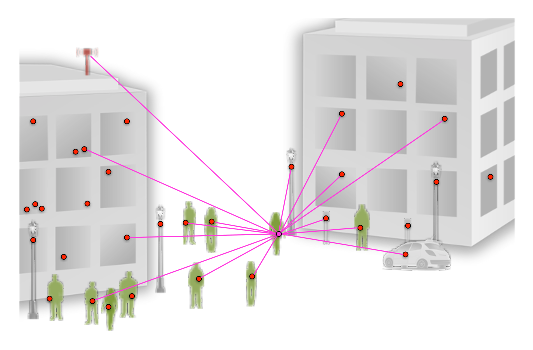
\includegraphics[width=0.8\textwidth]{res/fig/iot.eps}%
  \caption[
    Possibile scenario di rete in contesto urbano.
  ]{
    Possibile scenario di rete in contesto urbano.

    \nameCref{fig:iot} ripresa da~\cite{7274429}.
  }%
  \label{fig:iot}
\end{figure}

L'approccio tradizionale per la realizzazione di sistemi in questo contesto è sempre stato dal punto di vista del singolo dispositivo,
il quale è preso come unità fondamentale, connessa con il mondo fisico e con gli altri device.
In questo punto di vista, l'insieme di tutti i comportamenti individuali delle unità determina il funzionamento del sistema.
Tale approccio, per quanto valido, può risultare limitante in sistemi distribuiti eterogenei, nei quali possono presentarsi diversi problemi legati all'organizzazione della rete
e alla sua gestione a causa delle dimensioni e delle differenze tra i dispositivi.
Tali problematiche, generalmente, vorrebbero essere gestite ad un livello di astrazione più elevato.

L'\emph{aggregate programming}, o \emph{programmazione aggregata}, costituisce un'alternativa all'approccio ``classico''
volta a semplificare la progettazione, creazione e manutenzione di sistemi distribuiti complessi.
La programmazione aggregata, infatti, ragiona su larga scala, cercando di spostare l'attenzione sul \emph{collettivo di dispositivi} che collaborano,
astraendo dai dettagli relativi al singolo device~\cite{7274429} per quanto possibile.
% a capo rimosso
% TODO: rifai
L'idea alla base è dunque di definire una modalità di deduzione del comportamento locale al singolo dispositivo a partire dal comportamento globale, di più alto livello,
effettuando un \emph{mapping da globale a locale}.
In contesti distribuiti, sono stati individuati principalmente due punti di vista a questo livello di astrazione~\cite{aggregatescala-pmldc2016}: locale o globale.
Il primo, detto anche \emph{device-centric} (\Cref{fig:device-centric}), fa riferimento alla computazione aggregata eseguita dal singolo dispositivo.
Questo può essere considerato il punto di vista tradizionale.

\begin{figure}[htbp]
  \centering
  % \includesvg[width=.5\textwidth]{res/fig/device-centric.svg}
  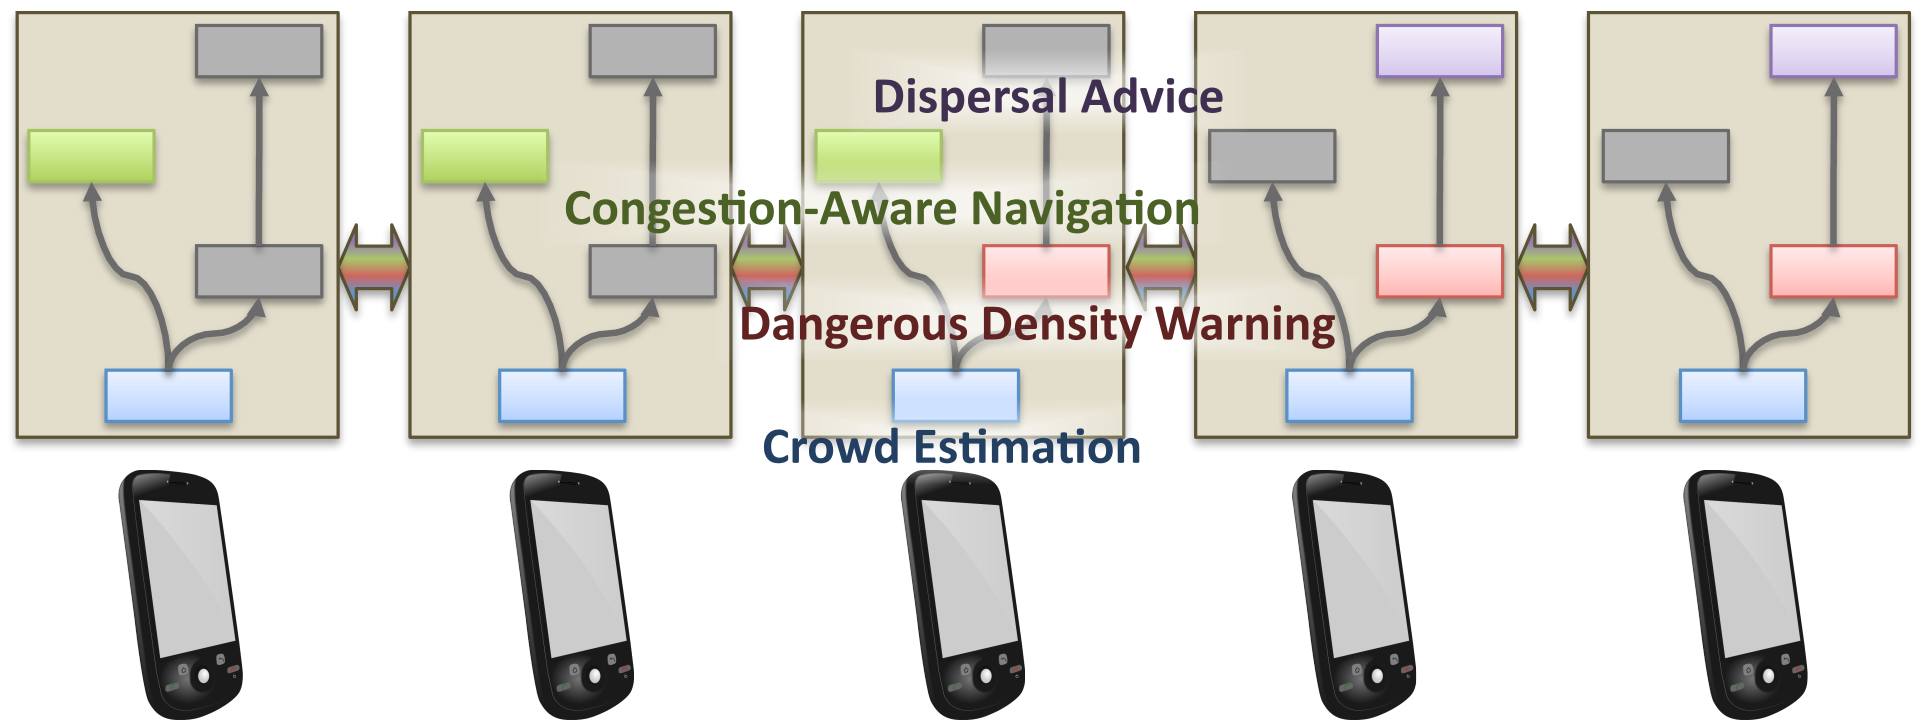
\includegraphics[width=.55\textwidth]{res/fig/device-centric.png}
  \caption{Livello di astrazione \emph{device-centric}}%
  \label{fig:device-centric}
\end{figure}

Il secondo punto di vista, detto \emph{aggregate view} (\Cref{fig:aggregate}), sposta invece l'attenzione sulla computazione svolta dal sistema aggregato come singola unità.
Rispetto all'approccio tradizionale, tale punto di vista sposta maggiormente l'attenzione dal \emph{come} il sistema possa funzionare
al \emph{cosa} effettivamente si desidera che faccia.

\begin{figure}[htbp]
  \centering
  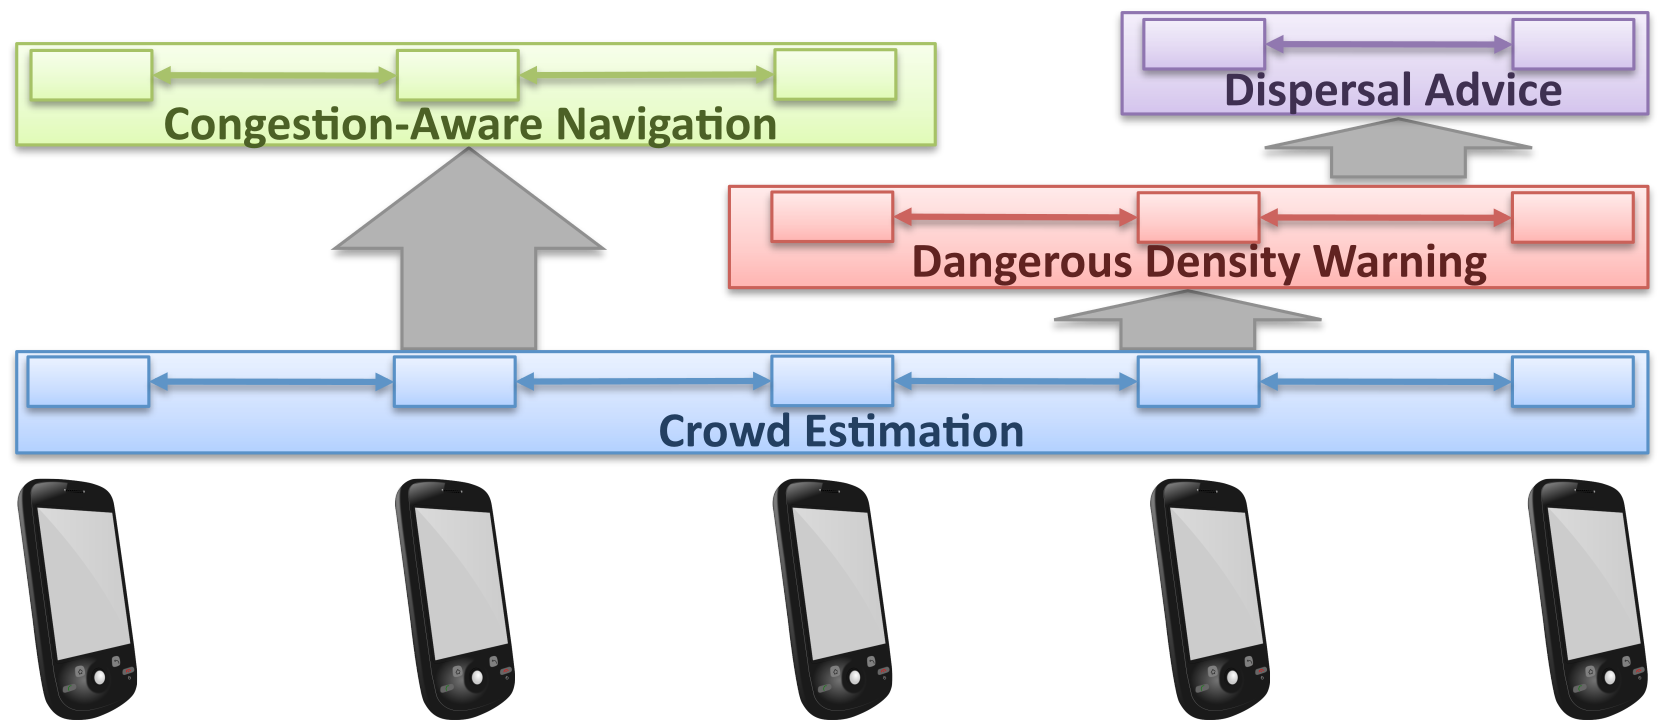
\includegraphics[width=.55\textwidth]{res/fig/aggregate.png}
  % \includesvg[width=.5\textwidth]{res/fig/aggregate.svg}
  \caption{Livello di astrazione \emph{aggregate view}}%
  \label{fig:aggregate}
\end{figure}

In letteratura, sono state adottate diverse strategie~\cite{7274429} ad un livello di astrazione così elevato.
Ad esempio, l'approccio \emph{TOTA} (``\emph{Tuples On The Air}''~\cite{10.1145/1538942.1538945}) prevede di rendere le interazioni tra i dispositivi implicite,
mentre l'\emph{Origami Shape Language}~\cite{nagpal2001programmable} si basa sulla composizione di costruzioni geometriche e topologiche attraverso operazioni di \emph{folding}.
Altri esempi sono le tecniche di sintesi dei dati provenienti da alcune regioni spazio-temporali per inviarli come stream ad altre regioni delineate con \emph{TinyDB}~\cite{1017485}
o le modalità con cui modelli di \emph{computazione cloud} come \emph{MapReduce}~\cite{10.1145/1327452.1327492} dividono la computazione in modo automatico tra i nodi.
Infine, linguaggi come \emph{Protelis}~\cite{PianiniSASOTutorial2017}, di cui tratteremo meglio in~\Cref{sec:protelis}, forniscono costrutti generalizzabili per la computazione spazio-temporale che si prestano ad un uso in ambiente IoT.

Lo studio dei suddetti approcci ha permesso di fare considerazioni sulle modalità di programmazione dei sistemi situati di larga scala;
innanzitutto, laddove non sia richiesto al programmatore di gestire i meccanismi di interazione, le modalità di coordinazione dovrebbero essere robuste e nascoste ``\emph{under the hood}''~\cite{7274429}.
Poi, il framework di programmazione dovrebbe essere modulare, e tali moduli dovrebbero essere componibili in modo semplice e trasparente.
Infine, deve essere possibile fornire meccanismi di coordinazione differenti per diverse parti del sistema aventi regioni dello spazio e tempi distinti.

La programmazione aggregata cerca di rispondere alle seguenti esigenze~\cite{7274429}:

% TODO: collassa elenco puntato
\begin{itemize}
  \item la ``macchina'' programmata non è il singolo dispositivo, bensì il loro agglomerato; % a \emph{regione} dell'ambiente computazionale che astrae dai dettagli specifici
  \item il ``programma'' è specificato come manipolazione di strutture dati distribuite che evolvono nel tempo dette \emph{computational fields};
  % TODO: modularità e componibilità
  \item tali manipolazioni vengono eseguite dai dispositivi inseriti all'interno della regione, tramite l'uso di meccanismi di coordinazione resilienti e di interazioni basate sulla prossimità.
\end{itemize}

In questo modo, i meccanismi di coordinazione, spesso complessi, vengono nascosti facilitando la costruzione e favorendo la modularità.
In particolare, il paradigma si struttura su più livelli di astrazione, come è possibile vedere in~\Cref{fig:stack}.

Nelle \nameCrefs{sec:field-calculus} successive analizzeremo più nel dettaglio alcuni di questi.

\begin{figure}[htbp]
  \centering
  \includesvg[width=0.55\textwidth]{res/fig/stack-2.svg}%
  \caption[
    Principali livelli dell'\emph{Aggregate Programming}.
  ]{
    Principali livelli dell'\emph{Aggregate Programming}.

    \nameCref{fig:stack} ripresa da~\cite{ProtelisSAC14}.
  }%
  \label{fig:stack}
\end{figure}

\section{Field calculus e Building Blocks}\label{sec:field-calculus}

Al livello più basso della struttura rappresentata in \Cref{fig:stack} si trova il \emph{field calculus}~\cite{tocl}.
Esso è un \emph{core calculus}, ovvero un modello teorico di programmazione che riassume la semantica operazionale minimale necessaria alla progettazione di un sistema aggregato.

Il field calculus si basato sul concetto di \emph{campo computazionale}~\cite{FieldCalculusFOCLASA2013,tocl}:
il termine riprende la nozione di campo in fisica~\cite{mcmullin2002origins}, esteso al concetto di computazione
e inteso come \enquote{\emph{una proiezione di ciascun dispositivo computazionale nello spazio verso un oggetto computazionale arbitrario}},
ossia l'applicazione di una funzione che, in un dato momento nel tempo, mappa ogni punto dello spazio (un dispositivo o un nodo),
verso un oggetto computazionale (un valore) che rappresenta il risultato della computazione su quel device.
I \emph{campi} sono strutture dati distribuite che si adattano ai cambiamenti della topologia sottostante e alle interazioni con l'ambiente.

I campi vengono generati e manipolati attraverso cinque costrutti fondamentali~\cite{tocl}:

\begin{description}

  \item[Operatori built-in] \((\,\texttt{b\,(e\textsubscript{1}\:\dots{}\:e\textsubscript{n})}\,)\) \\
    Un operatore \emph{built-in} \texttt{b} modella in modo uniforme operazioni basate su valori puntuali, cioè che non coinvolgono né lo stato, né la comunicazione.
    Esso determina il valore del campo in output all'evento \texttt{m} (un punto nello spazio-tempo) solo dai valori dello spazio \texttt{e}
    e dei campi in input \(\texttt{e\textsubscript{1}\:\dots{}\:e\textsubscript{n}}\).
    Possono essere funzioni \emph{stateless} matematiche, logiche o algoritmiche, ma anche sensori, attuatori, funzioni di libreria, ecc.

  \item[Definizione e chiamata di funzione] \((\,\texttt{def\ f\,(x\textsubscript{1}\:\dots{}\:x\textsubscript{n})\ e}\,)\) \\
    Astrazione e ricorsione sono supportate attraverso la definizione di funzione:
    una funzione \texttt{f} con parametri formali \(\texttt{x\textsubscript{1}\:\dots{}\:x\textsubscript{n}}\) e corpo \texttt{e}
    può essere invocata con \((\,\texttt{f\,(e\textsubscript{1}\:\dots{}\:e\textsubscript{n})}\,)\).

  \item[Evoluzione nel tempo] \((\,\texttt{rep\ x\;e\textsubscript{0}\;e}\,)\) \\
    Il costrutto di ripetizione supporta l'evoluzione dinamica dei campi, assumendo che ciascun dispositivo computi il proprio programma ripetutamente in \emph{round} asincroni.
    La variabile di stato \texttt{x} è inizializzata con il risultato della valutazione dell'espressione \texttt{e\textsubscript{0}} e aggiornato ad ogni step computando \texttt{e} in relazione al precedente valore di \texttt{x}.

  \item[Valori di vicinato] \((\,\texttt{nbr\ e}\,)\) \\
    L'interazione diretta tra i dispositivi è incapsulata nel costrutto \texttt{nbr};
    con esso, si ottiene il \emph{neighbouring field}, ossia una mappa da ciascun vicino al proprio valore corrente di \texttt{s}.
    Funzioni ``\emph{hood}'' \emph{built-in} possono poi riassumere queste mappe.

  \item[Restrizione di dominio] \((\,\texttt{if\ e\textsubscript{0}\;e\textsubscript{1}\;e\textsubscript{2}}\,)\) \\
    La ramificazione distribuita è implementata dal costrutto \texttt{if}, che permette di suddividere la rete in due regioni:
    una nella quale l'espressione \texttt{e\textsubscript{0}} è vera, nel quale \texttt{e\textsubscript{1}} viene computato, e una nella quale è falsa, che invece computerà \texttt{e\textsubscript{2}}.
    Tali suddivisioni sono incapsulate e non possono avere effetti al di fuori dei relativi sottospazi.
\end{description}

Questi costrutti permettono al \emph{field calculus} di essere universale~\cite{10.1007/978-3-319-92408-3_1},
supportando ogni computazione spazio-temporale causale e approssimabile.
Tramite questi operatori, inoltre, sono garantite \emph{portabilità}, \emph{indipendenza} dall'infrastruttura e \emph{integrazione} con servizi non aggregati.

Per poter garantire anche \emph{resilienza} alla coordinazione, è necessario introdurre il livello di astrazione successivo:
gli operatori ``\emph{building block}''~\cite{BV-FOCAS2014}.

Questo layer consiste di un insieme di operatori generici e di più alto livello, che offrono allo sviluppatore un ambiente di programmazione più espressivo,
contribuendo in particolare alla cosiddetta \emph{self-stabilization}, ossia la capacità di raggiungere uno stato atteso in un numero finito di passi,
indipendentemente dallo stato di partenza.
Tale proprietà è garantita per tutti i campi ottenuti tramite composizione funzionale~\cite{BV-FOCAS2014}.

\begin{figure}[htbp]
  \centering
  \includesvg[width=0.8\textwidth]{res/fig/stack-detail-crop.svg}%
  \caption{Dettaglio dei livelli più bassi dell'\emph{aggregate programming}.}%
  \label{fig:stack-detail}
\end{figure}

Come riportato in~\Cref{fig:stack-detail}, i \emph{building block} individuati in aggiunta al costrutto \texttt{if} del \emph{field calculus} sono tre operatori di coordinazione~\cite{7274429,BV-FOCAS2014}:

\begin{description}
  \item[Diffusione dell'informazione nello spazio]
    Letteralmente \enquote{diffusione dell'informazione nello spazio},
    quest'operatore generalizza operazioni molto comuni come la stima della distanza e messaggi broadcast.
    È definito come:

    \(\texttt{G\,(source,\:init,\:metric,\:accumulate)}\)

  \item[Raccoglimento di informazione attraverso lo spazio]
    Letteralmente \enquote{raccoglimento di informazione attraverso lo spazio},
    quest'operatore aggrega le informazioni verso la sorgente attraverso il gradiente di un campo specificato.
    È definito come:

    \(\texttt{C\,(potential,\:accumulate,\:local,\:null)}\)

  \item[Riassunto dell'informazione nel tempo]
    Letteralmente \enquote{riassunto dell'informazione nel tempo},
    quest'operatore generalizza un timer il cui rateo di aggiornamento può variare nel tempo.
    È definito come:

    \(\texttt{T\,(init,\:floor,\:decay)}\)
\end{description}

Questi operatori sono sufficientemente espressivi da poter coprire, da soli o combinati tra loro, molti dei pattern di coordinazione usati nei sistemi a larga scala.

Come livello di astrazione ulteriore (il secondo dall'alto nella~\Cref{fig:stack}), volto a semplificare la composizione dei \emph{building blocks}, si aggiungono le \emph{API general-purpose}~\cite{amslaurea13090}.
Esse possono essere usate e composte tra loro per scrivere applicazioni distribuite senza preoccuparsi dei meccanismi di coordinazione, la cui robustezza è garantita dagli operatori descritti sopra.

\section{Protelis}\label{sec:protelis}

% \begin{wrapfigure}{r}{0.2\textwidth}
%   \begin{center}
%     
\includegraphics[width=0.2\textwidth]{res/fig/protelis-logo.png}%
%     \caption{Logo}%
%     \label{fig:protelis}
%   \end{center}
% \end{wrapfigure}

% \begin{wrapfigure}{r}{0pt}
%   \centering
%   % \vspace{-52pt}
%   
\includegraphics[width=0.2\textwidth]{res/fig/protelis-logo.png}
%   % \vspace{50pt}
%   \caption{Logo}%
%   \label{fig:protelis}
% \end{wrapfigure}

Field calculus è un impianto teorico sul quale devono essere costruiti linguaggi ``pratici''.
Vista la necessità di un'architettura portabile in grado di gestire gli aspetti di comunicazione, esecuzione e interfacciamento con hardware e sistema operativo, è stato realizzato Protelis.

\emph{Protelis}~\cite{PianiniSASOTutorial2017} è un linguaggio di programmazione basato sul paradigma aggregato fortemente influenzato da \emph{Proto}~\cite{Beal2006}.
Il linguaggio incorpora le principali funzionalità di computazione spaziale di field calculus in una sintassi più simile ai linguaggi strutturati tradizionali come C o Java.

\begin{figure}[htbp]
  \centering
  \includesvg[width=0.4\textwidth]{res/fig/protelis-abstract-arch.svg}
  \caption[
    Architettura di Protelis
  ]{
    Architettura di Protelis.

    Figura ripresa da~\cite{ProtelisSAC14}.
  }%
  \label{fig:protelis-stack}
\end{figure}

% \begin{wrapfigure}{l}{0pt}
%   \centering
%   \includesvg[width=0.4\textwidth]{res/fig/protelis-abstract-arch.svg}
%   \caption{Architettura di Protelis}%
%   \label{fig:protelis-stack}
% \end{wrapfigure}

Un nodo Protelis è costituito da un \emph{parser} che traduce il programma in codice eseguibile, il quale è poi eseguito a intervalli regolari da un \emph{interprete}, che si fa carico degli aspetti di interazione con il vicinato e con l'ambiente.
Ogni esecuzione è chiamata \emph{computational round}.

Il linguaggio e l'interprete sono basati su Java e possono essere inseriti in contesti virtuali~\cite{ProtelisSAC14} o reali indifferentemente~\cite{AggregatecomputingVlsubicomp16}.
Questo offre, da un lato, la portabilità e il supporto alle differenti piattaforme che la JVM (\emph{Java Virtual Machine}) mette a disposizione, dall'altro l'estendibilità che l'ecosistema di librerie Java può offrire.

Nel mondo scientifico, il linguaggio è già stato utilizzato per la realizzazione di diversi algoritmi aggregati.
Di seguito sono riportati alcuni esempi.

\begin{description}
  \item[Algoritmi legati all'affollamento]
    Tramite Protelis, è stato possibile~\cite{7274429} stimarne la pericolosità di una data zona nell'ambiente basandosi sulla densità dei dispositivi presenti e definire modalità di dispersione efficaci.

    In un altro progetto~\cite{DBLP:journals/fgcs/CasadeiFPRSV19}, è stata definito un algoritmo di \emph{rendezvous} in grado di evitare le zone ad alta densità nel contesto di un evento di massa, permettendo l'incontro di due individui in un punto intermedio.

  \item[Gestione di reti di servizi]
    Un altro utilizzo significativo è stato per la realizzazione di un sistema di gestione tra servizi in rete.
    Tali servizi, talvolta datati, possono avere molte dipendenze tra loro e scarse capacità di coordinazione.
    Per evitare stati di inconsistenza, spesso l'ordine di arresto dei server è strettamente legato alle dipendenze e rende difficile l'automazione.

    Utilizzando Protelis è stato possibile~\cite{7306601} realizzare un sistema in grado di organizzarsi per riavviare lo stack.
    In particolare, sono state definite entità chiamate \emph{daemon} che monitorano ciascuna uno specifico servizio e comunicano con le altre al fine di garantire l'ordine necessario.

  \item[Integrazione con servizi di realtà aumentata]
    La programmazione aggregata è stata testata anche nell'ambito dell'AR (\emph{Augmented Reality})~\cite{PCRV-SCOPES2015}.

    Ad esempio, è possibile utilizzare visori di realtà aumentata per visualizzare nell'ambiente i campi computazionali
    o, viceversa, modellare i dati raccolti da sensori AR come campi (detti \emph{augmented fields}).
\end{description}

\section{ScaFi}\label{sec:scafi}

Una tecnologia analoga è rappresentata da \emph{ScaFi} (\emph{\emph{Sca}la with computational \emph{Fi}elds})~\cite{aggregatescala-pmldc2016}:
si tratta di un framework in Scala per la realizzazione di programmi aggregati attraverso un set compatto di primitive, presentato come implementazione del field calculus alternativa a Protelis.
% Nonostante sia dunque un DSL di Scala, è sufficientemente completo da poter essere considerato un linguaggio di programmazione aggregata a sé stante.

Il framework è composto principalmente da due parti:

\begin{description}
  \item[Aggregate programming support]
    La prima parte è un \emph{internal DSL} (\emph{Domain Specific Language}) di Scala che fornisce la sintassi e la semantica per i costrutti base del field calculus.

  \item[Aggregate platform support]
    La seconda parte è una piattaforma distribuita basata sul modello ad attori di Akka che permette la configurazione e l'esecuzione di sistemi aggregati.
    Essa può essere utilizzata in modalità decentralizzata (\emph{peer-to-peer}) %, \Cref{fig:scafi:p2p}
    o in modalità centralizzata (\emph{server-based}).%, \Cref{fig:scafi:server-based}                  % ChkTeX 37

    % \begin{figure}[htbp]
    %   \centering
    %   \begin{subfigure}{0.35\textwidth}
    %     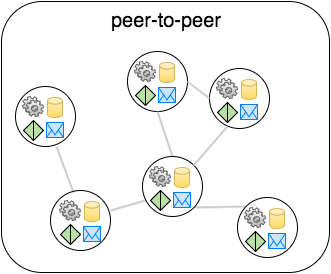
\includegraphics[width=\textwidth]{res/fig/scafi-p2p.png}
    %     \caption{Architettura \emph{peer-to-peer}}%
    %     \label{fig:scafi:p2p}
    %   \end{subfigure}
    %   \hspace{0.15\textwidth} % a differenza di \hfill il commento serve per non aggiungere spazi
    %   \begin{subfigure}{0.35\textwidth}
    %     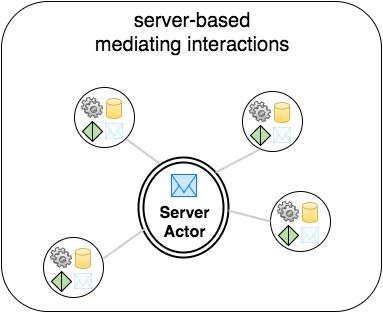
\includegraphics[width=\textwidth]{res/fig/scafi-server-based.png}
    %     \caption{Architettura \emph{server-based}}%
    %     \label{fig:scafi:server-based}
    %   \end{subfigure}
    %   \caption[
    %     Architetture della piattaforma distribuita di ScaFi
    %   ]{
    %     Architetture della piattaforma distribuita di ScaFi.

    %     Figura ripresa da~\cite{AggregatecomputingVlsubicomp16}.
    %   }%
    %   \label{fig:scafi}
    % \end{figure}

    Nel caso centralizzato, è la piattaforma a mantenere le posizioni spaziali dei dispositivi e a gestire il vicinato, secondo il modello tradizionale client-server.
\end{description}

Dato che si appoggia su Scala come linguaggio ospite, è in grado di interoperare con Java e gli altri linguaggi in grado si eseguire in ambiente JVM, mantenendo il solido \emph{type-system} messo a disposizione da Scala e i suoi costrutti funzionali.

    \chapter{Progettazione di sistemi web}\label{ch:web}
  Il World Wide Web ha assunto un ruolo sempre più centrale nella quotidianità delle persone e nelle dinamiche di business.
  In particolare, il modello di comunicazione è sempre più virato verso scenari distribuiti,
  nei quali piattaforme eterogenee riescono a comunicare tra loro condividendo informazioni di diverso tipo attraverso la rete internet.

  Anche i pattern di progettazione e le tecnologie implementative sono cresciute altrettanto velocemente negli ultimi anni, cambiando anche radicalmente gli approcci di interazione possibili.
  Risulta dunque importante prestare attenzione allo stato dell'arte in tal senso, chiarendo quali siano i pattern più adatti e moderni per il contesto d'uso di questa tesi.

  \section{Architetture \& paradigmi}\label{sec:web-architecture}

  Con \emph{sistema web} si intende genericamente un sistema software distribuito che coinvolge una o più entità server che espongono in rete API di varia natura, con le quali entità client possono comunicare per usufruire dei servizi.
  Generalmente, in contesto web i client sono costituiti da pagine web aperte nei browser degli utenti.

  Le possibilità di progettazione di un'applicazione web possono essere molto differenti e nel tempo si è vista una vera e propria evoluzione in tal senso.

  % \begin{enumerate}
  %   \item
  %     Nel periodo iniziale del web, ciascuna pagina web era inviata al client come un documento statico;
  %     l'interazione dell'utente con il sistema avveniva attraverso la navigazione, che comportava l'apertura di una sequenza di pagine a seconda delle esigenze.
  %     Questo tipo di interazione era però lenta, in quanto coinvolgeva sempre la ricezione di una nuova pagina dal server.
  %   \item
  %     Successivamente, nel 1995, con l'introduzione da parte di NetScape di JavaScript (di cui tratteremo meglio nella~\Cref{subsec:js}) come linguaggio di scripting client-side, i programmatori hanno avuto la possibilità di inserire elementi dinamici nelle pagine web.
  %     In questo modo, era possibile effettuare alcune operazioni anche localmente, riducendo di fatto il numero di pagine intere scambiate con il server.
  %   \item
  %     Un'ulteriore innovazione apparve l'anno seguente, quando Macromedia introdusse \emph{Flash}:
  %     esso era un plugin per i browser che permetteva di riprodurre animazioni vettoriali e gestire le interazioni con l'utente, in modo simile a quanto fatto da JavaScript.
  %   \item
  %     Il termine ``\emph{web application}'' nasce però con l'introduzione della versione 2.2 della Java Servlet Specification~\cite{java1999specification} nel 1999.
  %     anche in questo caso, però, il server ha un ruolo centrale e ancora il concetto di \emph{ajax} (\emph{Asynchronous JavaScript + XML}) non è stato introdotto.
  %   \item
  %     Successivamente vi sono stati diversi miglioramenti incrementali, fino ad arrivare allo standard HTML5~\cite{Smith2008}:
  %     quest'ultimo, infatti, introduce il supporto nativo ai contenuti multimediali ed arricchisce la semantica del documento, oltre a migliorare l'integrazione con JS\@.
  %     Con questo standard, diventa sempre più comune il concetto di \emph{Single-page application} (SPA), secondo il quale la pagina viene caricata una sola volta, e poi modificata dinamicamente tramite chiamate specifiche al server.
  %     Nascono numerosi framework client-side (come Angular, Ember o React) e l'impiego del server viene sempre più circoscritto al fornire API per accesso controllato ai dati (ad esempio, un database) o per computazioni complesse.
  % \end{enumerate}

  Nel periodo iniziale del web, ciascuna pagina era inviata al client come documento statico;
  in questo caso, i server si occupavano della computazione di quanto richiesto dall'utente (anche appoggiandosi a servizi esterni tramite \emph{Common Gateway Interface}~\cite{Coar2004}) e della composizione del documento.

  Nel corso degli anni, sono stati sviluppati linguaggi di scripting (come JavaScript e Macromedia Flash) in grado di aumentare le possibilità di interazione lato client, riducendo la quantità di dati trasferiti tra il server web e il browser:
  non viene infatti più scaricata una nuova pagina ad ogni azione dell'utente, bensì solo i dati richiesti tramite chiamate \emph{AJAX} (\emph{Asynchronous JavaScript And XML});
  il documento viene poi manipolato localmente inserendo i dati ricevuti.

  Con l'avvento di HTML~5~\cite{Smith2008}, viene introdotto il supporto nativo ai contenuti multimediali ed arricchita la semantica del documento;
  inoltre JavaScript riceve un supporto di prima classe e la necessità di plugin esterni come Flash diminuisce.

  Vengono sviluppati numerosi framework per la realizzazione di applicazioni costituite da una singola pagina (\emph{SPA}, \emph{Single-Page Application}), in grado di offrire l'esperienza d'uso di un applicativo desktop.
  Un applicazione web moderna normalmente è di questo tipo.

  \improvement[inline]{Dovrei aggiungere qualche immagine per ridurre l'effetto wall-of-text?}

  \improvement[inline]{
    Inizialmente avevo inserito una storia dell'evoluzione delle architetture client-side e \strong{server-side}, ma poi mi sono reso conto che risultava un po' fuori contesto e l'ho tolta.

    Ritenete invece che potesse avere il suo senso come background? Nel caso posso reintegrarla velocemente.
  }

  % % Se inizialmente il server web si occupava dell'intero processo di costruzione della pagina, un po' alla volta le operazioni da effettuare per l'invio si sono sempre più ridotte.

  % % \begin{figure}[htbp]
  % %   \centering
  % %   \includesvg[width=.8\textwidth]{res/fig/server-evolution.svg}
  % %   \caption{Il controllo sulla costruzione della pagina si è spostato sempre più verso il client}%
  % %   \label{fig:server-evolution}
  % % \end{figure}

  % % In applicazioni l server diventa sempre più dedicato al memorizzare i dati (tramite database, ad esempio) e il codice client, mentre il browser si occupa di buona parte della logica applicativa.
  % Il primo approccio alla gestione della logica applicativa via rete fu quello di demandare la generazione dei contenuti a processi esterni tramite l'interfaccia standard CGI (\emph{Common Gateway Interface}~\cite{Coar2004}).
  % Essa permetteva al web server di lanciare un processo per ogni richiesta, passando i parametri necessari per l'elaborazione e di ricevere il risultato.
  % L'approccio era però poco scalabile e molto pesante per le risorse.

  \section{Linguaggi ad uso web}\label{sec:lang}
    In questa \nameCref{sec:lang} verranno analizzati i principali linguaggi di programmazione utilizzati recentemente per lo sviluppo della componente frontend delle applicazioni web.
    In particolare, verranno presi in considerazione i due linguaggi più popolari in questo contesto, ossia \emph{JavaScript} e il suo super-set \emph{TypeScript}, e due linguaggi non nativi della piattaforma che possono offrire una valida alternativa:
    \emph{Scala.js} e \emph{Kotlin/JS}\@.

    \subsection{JavaScript e ECMAScript}\label{subsec:js}

      % \begin{wrapfigure}{r}{0pt}
      %   \centering
      %   % \vspace{-52pt}
      %   \includesvg[width=0.2\textwidth]{res/fig/js-logo.svg}
      %   % \vspace{50pt}
      %   \caption{Logo}%
      %   \label{fig:js}
      % \end{wrapfigure}

      \emph{JavaScript} è un linguaggio di scripting debolmente tipizzato multi-paradigma, con supporto agli stili di programmazione % funzionale, ad eventi, orientato agli oggetti.
      \begin{inparaitem}
        \item funzionale,
        \item ad eventi,
        \item orientato agli oggetti.
      \end{inparaitem}
      Sviluppato originariamente nel 1995 da Brendan Eich per Netscape Communications (inizialmente con il nome di \emph{Mocha} e poi \emph{LiveScript}),
      esso è stato concepito con lo scopo di avere un linguaggio di scripting per il browser Netscape Navigator più semplice da apprendere rispetto a quelli esistenti.
      JavaScript è stato standardizzato per la prima volta nel 1997 dalla ECMA con il nome di \emph{ECMAScript}~\cite{ECMA-262,ISO:1998} e l'attuale versione è la decima.

      Il linguaggio è attualmente il più popolare per uso web, in quanto l'unico ad essere supportato da tutti i browser moderni, almeno nelle sue feature principali.
      Diversi linguaggi, come quelli che vedremo in seguito, vengono transcompilati in una versione sufficientemente supportata di JS da poter essere eseguiti nei browser.

      Analizzato dal punto di vista tecnico, esso presenta i seguenti aspetti strutturali:

      \begin{description}
        \item[Imperativo e strutturato]
          Il linguaggio si presenta con una sintassi di programmazione strutturata standard, con il supporto a tutte le strutture di controllo tradizionali.
          Una parziale differenza era nella gestione della visibilità delle variabili (\emph{scope}):
          inizialmente, JavaScript garantiva solo la visibilità a livello di funzione (\emph{function scope}) tramite la parola chiave \texttt{var};
          con ECMAScript 6 è stato aggiunto il supporto alla visibilità a livello di blocco (\emph{block scope}).

        \item[Tipizzazione dinamica]
          % https://developer.mozilla.org/en-US/docs/Web/JavaScript/Data_structures
          JavaScript è un linguaggio debolmente tipizzato:
          alle variabili non sono associati dei tipi di dato, ma solo dei valori, che possono dinamicamente cambiare tipo durante il ciclo di vita della variabile.
          La tipizzazione dinamica consente lo stile di tipizzazione chiamato \emph{duck typing}~\cite{10.1145/2103621.2103686} (o \emph{structural subtyping}):
          è possibile determinare la semantica di un oggetto in base ai metodi ed alle proprietà che esso possiede,  non in base al suo tipo.

        \item[Orientamento agli oggetti Prototype-based]
          A differenza di altri linguaggi orientato agli oggetti (come Java o C++), JavaScript non fornisce un'implementazione del concetto di \emph{classe}~\cite{Ungar1991}:
          la stessa keyword \texttt{class}, introdotta con ES6, non è altro che zucchero sintattico per migliorare l'interazione da parte degli sviluppatori con il prototipo dell'oggetto.

          In termini di ereditarietà, infatti, JS prevede un solo costrutto: gli \emph{oggetti}.
          Ogni oggetto ha un collegamento interno ad un altro oggetto chiamato \emph{prototype}.
          Questo oggetto prototipo ha a sua volta un suo prototype, e così via finché si raggiunge un oggetto con la proprietà prototipo settata a \texttt{null}.
          Per definizione, \texttt{null} non ha un prototype ed agisce come anello finale nella \emph{catena di prototipi}.

          Quasi tutti gli oggetti in JavaScript sono istanze di \texttt{Object}, che risiede in cima alla catena dei prototipi.
          % In JavaScript, è possibile aggiungere proprietà a qualsiasi oggetto in fase di esecuzione.

        \item[First-class function]
          JavaScript offre un supporto di prima classe alle funzioni, che sono considerate oggetti;
          come tali, esse possono avere delle proprietà, come ad esempio \texttt{.bind()} e \texttt{.call()}. % ChkTeX 36

          Ciascuna funzione costituisce una \emph{chiusura lessicale}.

          All'interno degli oggetti, le proprietà di tipo funzione vengono utilizzate come costruttori e come metodi.
          Infine, le funzioni possono essere utilizzate anche per l'implementazione di \emph{pattern di ruolo} come i \emph{tratti} e i \emph{mixin}.

        \item[Web APIs]
          Con ECMAScript si standardizza la componente \emph{core} del linguaggio, che può eseguire in ambienti browser come su interpreti non legati strettamente al web (come ad esempio Node.js~\cite{5617064}).
          Ciascuno degli ambienti nei quali il linguaggio viene interpretato mettono a disposizione delle API specifiche per l'interazione con la piattaforma;
          quando si fa riferimento al browser, tali supporti sono chiamati \emph{Web APIs}.

          Attraverso di esse, lo sviluppatore può avere accesso agli elementi del DOM (Document Object Model) di HTML, potendo manipolare la pagina visualizzata e reagire ad eventi su di essa.

        \item[Asincronismo]
          JavaScript supporta inoltre nativamente l'esecuzione di operazioni in modo asincrono tramite il costrutto della \emph{promise}, implementato da un oggetto built-in \texttt{Promise},
          che costituisce un \emph{proxy} per un valore non necessariamente noto quando la promise viene creata.
          È poi possibile gestire il valore ottenuto con costrutti ``\emph{thenable}'' o con il \emph{pattern async/await}.
      \end{description}

    \subsection{TypeScript}\label{subsec:ts}
      \emph{TypeScript} è un linguaggio di programmazione open-source sviluppato da Microsoft.
      Esso è un super-set sintatticamente rigoroso di JavaScript ES6, nato con i seguenti obiettivi principali:

      \begin{itemize}
        \item
          l'introduzione di funzionalità \emph{cutting-edge} (talvolta anche nei primi stage di approvazione) di ECMAScript.
          Esse sono rese disponibili transcompilando il sorgente TypeScript in codice JavaScript meno recentemente ma completamente compatibile con l'ambiente di esecuzione scelto
          (ad esempio ES5 per i browser), spesso avvalendosi di \emph{polyfill} per estendere la compatibilità.
          Tra queste funzionalità, ci sono ad esempio:
          \begin{description}
            \item[Decoratori]
              Definiti in una proposta ECMAScript~\cite{decorators} tutt'ora pendente (stage 2 al momento della scrittura),
              i decoratori sono dichiarazioni (definite tramite carattere ``\texttt{@}'') associate a una dichiarazione di classe, un metodo, una proprietà o un parametro che permettono la valutazione a runtime di una espressione specificata.
              Il framework Angular, ad esempio, utilizza estensivamente questa funzionalità per effettuare \emph{dependency injection}.

            \item[Operatore di coalescenza del null \& safe navigation]
              In JavaScript, sono considerati \emph{falsy} valori come \texttt{NaN}, \texttt{0} e la stringa vuota che, pur non essendo \texttt{null} o \texttt{undefined},
              vengono trattati come valori ``non presenti'' e dunque come \texttt{false} dagli operatori booleani.
              Per ridurre la possibilità di bug dovuto a questo tipo di valori, sono stati definiti gli operatori di \emph{nullish coalescing} ``\texttt{??}'' e di \emph{safe navigation} ``\texttt{.?}''.
              Definiti sulla base di una precedente proposta ECMAScript~\cite{optional}, solo più tardi integrata, sono stati introdotti con la versione 3.7 di TypeScript.
          \end{description}
        \item
          l'introduzione di un sistema di \emph{tipizzazione statica} opzionale che possa integrarsi nel modo più trasparente possibile nella sintassi JavaScript standard;
          in particolare, viene data la possibilità di definire tipi complessi tramite \emph{sintassi postfissa}.
      \end{itemize}

      % Di fatto, dunque, presenta tutte le caratteristiche di JavaScript descritte nella \Vref{subsec:js}.
      Il sistema di tipi viene presentato come \emph{class-based} (in contrapposizione al \emph{prototype-based} tipico di JavaScript, soprattutto prima dell'introduzione dello zucchero sintattico per le classi), ma mantiene le caratteristiche di structural subtyping citate precedentemente.
      Avvalendosi di ciò, il linguaggio permette la definizione di tipi complessi;
      è garantito il supporto ai generici, esteso da un'algebra dei tipi molto flessibile che permette unione, intersezione e condizionalità, oltre alla possibilità di accesso ai tipi delle singole proprietà.

      La generazione dei metadati per la descrizione dei tipi permette un'integrazione migliore di TypeScript e JavaScript con gli ambienti di sviluppo;
      inoltre, negli anni è diventato lo standard de-facto per la documentazione dei moduli per il linguaggio, sostituendo le soluzioni basate sul parsing dei commenti come JSDoc.

    \subsection{Scala.js}\label{subsec:scalajs}
      \emph{Scala.js} è un compilatore per il linguaggio di programmazione Scala che genera codice JavaScript invece di bytecode per la JVM\@.
      % Questo permette l'impiego di tutte le funzionalità di Scala in contesto web, massimizzando il riuso di codice condiviso con la componente backend potenzialmente scritto con il medesimo linguaggio e in esecuzione su JVM\@.

      I principali vantaggi dell'impiego di un linguaggio come Scala all'interno del contesto web sono i seguenti:
      \begin{description}
        \item[Struttura più solida]
          Come detto, JavaScript è un linguaggio debolmente tipizzato;
          se questo aggiunge notevole flessibilità durante lo sviluppo, d'altro canto aggiunge una maggiore possibilità di bug.
          Anche TypeScript, che offre un sistema di tipi molto più completo, risulta talvolta anomalo per via della natura strutturale della tipizzazione implementata.

          Scala mette a disposizione un type system allo stesso tempo più espressivo e più rigoroso, di conseguenza può risultare più \emph{user-friendly} sia durante lo sviluppo che in fase di debug.

        \item[Prestazioni]
          Secondo benchmark~\cite{Doeraene:256862} realizzati tramite una suite estensiva già utilizzata in letteratura~\cite{10.1145/3093334.2989232}, per quanto Scala.js risulti più lento della controparte JVM, riesce ad essere fino al 33\% più veloce della controparte scritta in JavaScript.

          Inoltre, il compilatore risulta molto efficiente in termini di dimensioni finali del \emph{bundle}:
          secondo il sito ufficiale, generalmente si parte dai \(\SI{45}{\kilo\byte}\) per un'intera applicazione compressa in gzip.
          Questo permette di avere buone performance al primo caricamento dell'applicazione web.

        \item[Interoperabilità con JavaScript]
          Scala.js è dichiaratamente compatibile con qualsiasi modulo JavaScript, purché sia dotato del codice \emph{façade} necessario per garantirne il type checking.
          Il team che mantiene il progetto ha effettuato il wrapping di numerose librerie di uso comune (50 al momento della scrittura) e mette a disposizione uno strumento di conversione automatico per le definizioni di tipo generate dal compilatore di TypeScript.
          Data la popolarità di quest'ultimo, la copertura può essere dunque considerata elevata.

        \item[Riuso]
          Un'altra compatibilità utile nella realizzazione di sistemi web di grandi dimensioni è quella con codice Scala impiegato anche nel backend.
          Questo permette di riutilizzare il codice condiviso tra server e client,
          riducendo i costi di manutenzione del medesimo codice in linguaggi differenti e la possibile \emph{friction} originata dall'etereogeneità dei linguaggi.

          Non è possibile riutilizzare codice che dipende strettamente da funzionalità della JVM (\emph{reflection}, eccezioni native di Java), in quanto porta a comportamenti indefiniti.
      \end{description}

      % Oltre al supporto semi-ufficiale a React e altri framework e librerie per la realizzazione di SPA, Scala offre un'integrazione di prima classe anche con tecnologie backend molto famose come il Play Framework di Lightbend.
      Scala inoltre ha un'integrazione molto buona con ambienti di sviluppo comunemente utilizzati, che può portare a una rilevazione degli errori più veloce e ad un autocompletamento più preciso.

    \subsection{Kotlin/Multiplatform \& Kotlin/JS}\label{subsec:kotlinjs}
      Con il rilascio della versione 1.1 di Kotlin nel 2017, JetBrains ha annunciato \emph{Koltin/JS}~\cite{Belov2017}, un target del compilatore in grado di generare codice JavaScript ES5 invece che bytecode per la JVM, in modo simile a quanto fatto da Scala.js.
      Il progetto si colloca in un progetto di più ampio respiro, ossia \emph{Kotlin/Multiplatform}~\cite{Jemerov2017}, presentato al termine dello stesso anno in concomitanza con Kotlin 1.2, che mira a integrare anche il supporto ad altri target, tra cui ad esempio LLVM\@.

      L'intento è molto simile a quello di Scala.js:
      fornire un linguaggio solido per la realizzazione di componenti web (ad esempio un frontend) con lo stesso codice in esecuzione sul server con cui dialogare, in modo da coprire l'intero sistema nel modo più omogeneo possibile.

      Kotlin, a differenza di quanto avviene in Scala.js, però, prevede l'utilizzo di sorgenti separati per la parte comune (\emph{common source set}), che modella il sistema in Kotlin puro, e per la parte specifica di ciascun particolare target:
      in questo modo, differenti piattaforme possono avere implementazioni più vicine alle rispettive native, avvalendosi di librerie specifiche fornite dal sistema o da terze parti.

      Anche in questo caso, le criticità sono simili a quelle citate nella \nameCref{subsec:scalajs} precedente:
      \begin{itemize}
        \item
          per quanto l'intera libreria standard sia stata portata da JetBrains sulle diverse piattaforme nel modo più trasparente possibile, le piattaforme di esecuzione rimangono differenti.
          Di conseguenza, alcuni costrutti molto specifici strettamente legati alla JVM (come ad esempio la reflection) non sono disponibili sul target JS\@.
        \item
          per garantire il supporto corretto ai tipi, è necessaria la presenza di codice \emph{wrapper} che li modelli.
          JetBrains ha realizzato gli adattamenti solo per poche librerie, principalmente legate a React, e ha messo a disposizione alcuni strumenti per la conversione delle definizioni di tipo di TypeScript.
          Purtroppo, la prima soluzione, \texttt{ts2kt}, è stata deprecata solo dopo qualche anno e il sostituto, \texttt{dukat}, al momento della scrittura non è ancora considerato stabile.

          In assenza dei wrapper, è comunque possibile lavorare con moduli JavaScript attraverso il costrutto \texttt{dynamic}, ma si perde il controllo sui tipi.
      \end{itemize}

      JetBrains pare supportare attivamente la libreria React per la realizzazione di codice frontend, ma attualmente non viene ritenuto ancora sufficientemente stabile per un uso reale.
      Sul sito ufficiale sono invece specificati numerosi framework per la realizzazione di backend che offrono supporto di prima classe al linguaggio.

    \chapter{Motivazioni}\label{ch:motivations}

  Come detto nell'\nameref{ch:intro}, il rapido aumento di dispositivi capaci di computare e distribuiti nell'ambiente ha reso necessario ideare nuovi paradigmi di programmazione.
  Uno di questi è senza dubbio l'\emph{aggregate programming}, di cui si è trattato nel dettaglio nel~\Cref{ch:aggregate}.

  In questo \nameCref{ch:motivations} verrà analizzato lo stato dell'arte relativamente alla creazione di un programma aggregato,
  mettendo in evidenza le ragioni per la quale è stato realizzato questo progetto di tesi.

  \section{Stato dell'arte}\label{sec:state-of-art}

  Prima di partire con la progettazione del sistema, è stato necessario valutare lo stato dell'arte nel quale il software va ad inserirsi.
  % Si è dunque deciso di analizzare nel dettaglio quali sono i punti critici dello stato dell'arte;
  % i
  In particolare, si è preso in considerazione la procedura di configurazione di un progetto realizzato in un linguaggio aggregato,
  confrontandolo con l'esperienza di sviluppo ottenuta con altri linguaggi in altri contesti.

  \subsection{Accessibilità allo sviluppo in Protelis}\label{subsec:setup}

  I due principali linguaggi di programmazione aggregata che implementano il modello teorico del field calculus sono Protelis e ScaFi.
  ScaFi è un DSL interno a Scala e, come tale, richiede di essere utilizzato all'interno di progetti basati su tale linguaggio;
  poiché sono già state realizzate tesi~\cite{amslaurea12188,amslaurea16824} incentrate sull'esecuzione di ScaFi,
  è stato richiesto di concentrarsi, in questa tesi, solamente su Protelis.

  Protelis è un linguaggio \emph{Java-hosted} e, come tale, deve essere caricato in un progetto JVM che esegue un'istanza del suo interprete.
  Di seguito sono riportate le possibili modalità di esecuzione documentate nello stato dell'arte.

  \begin{description}
    \item[Alchemist]\cite{ProtelisSAC14}
      Una prima possibilità di utilizzo è tramite il simulatore Alchemist~\cite{alchemist-jos2013}.
      Esso mette infatti a disposizione all'interno del proprio meta-modello un'incarnazione specifica per Protelis.
      Esso permette la simulazione di reti con pattern anche complessi con semplici file di configurazione.
      In~\Cref{fig:alchemis-protelis} sono riportate le entità in gioco.

      \begin{figure}[htbp]
        \centering
        \includesvg[width=0.52\textwidth]{res/fig/protelis-alchemist-arch.svg}%
        \caption[
          Implementazione dell'architettura di Protelis in Alchemist
        ]{
          Implementazione dell'architettura di Protelis in Alchemist.

          \nameCref{fig:alchemis-protelis} ripresa da~\cite{ProtelisSAC14}.
        }%
        \label{fig:alchemis-protelis}
      \end{figure}

      Alchemist può essere utilizzato all'interno di altro software in ambiente Java come libreria di virtualizzazione, oppure in modo indipendente tramite linea di comando\footnote{\url{https://github.com/Protelis/Protelis-Alchemist-tutorial}}.
      In questo secondo caso, è possibile definire il codice Protelis insieme a file di configurazione in formato YAML e specificarli al lancio del file jar eseguibile di Alchemist.
      Il simulatore mette a disposizione un'interfaccia grafica minimale per la visualizzazione e il controllo della simulazione.

    \item[ProtelisVM]\cite{amslaurea19778}
      Un'altra possibilità è tramite l'importazione del framework di Protelis nel \emph{classpath} di un progetto Java, ad esempio prelevandolo come dipendenza Maven.
      Il framework mette a disposizione una classe denominata \texttt{ProtelisVM} (\Cref{fig:protelisvm}), che si occupa di eseguire un programma Protelis in un \texttt{ExecutionContext},
      ossia un'astrazione del dispositivo esecutore che si frappone tra la macchina virtuale e l'ambiente fisico.

      \begin{figure}[htbp]
        \centering
        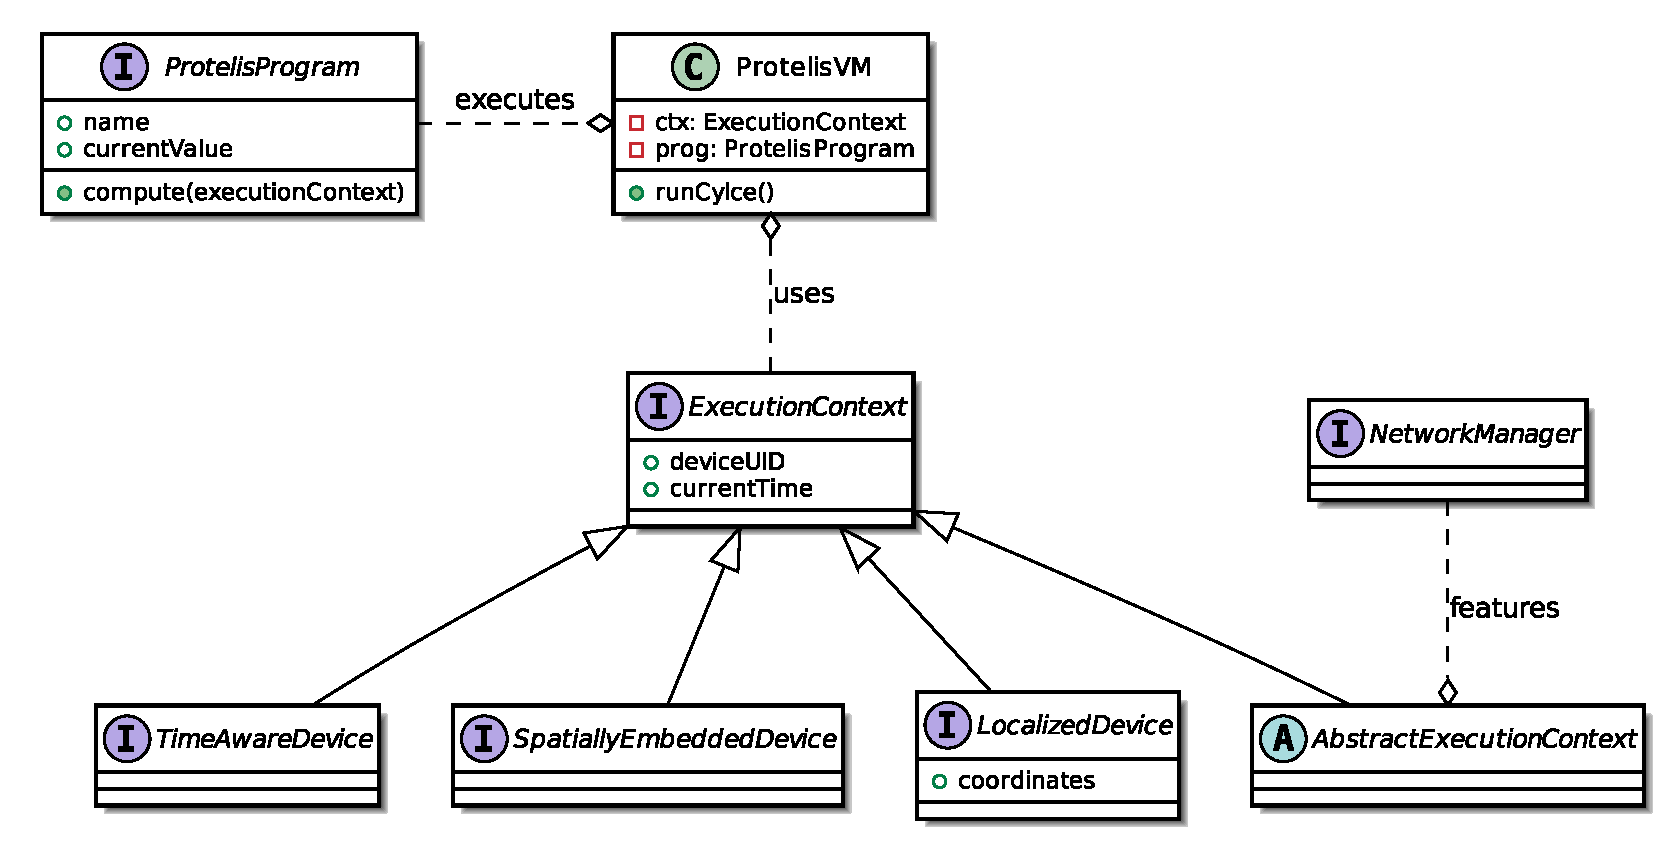
\includegraphics[width=0.87\textwidth]{res/uml/ExecutionContext.eps}%
        \caption{UML delle principali entità del framework di Protelis}%
        \label{fig:protelisvm}
      \end{figure}

      Attraverso la libreria è possibile definire dispositivi virtuali o, potenzialmente, collegare implementazioni fisiche.
      Su GitHub\footnote{\url{https://github.com/Protelis/Protelis-Demo}} sono riportati alcuni esempi con diverse opzioni di integrazione.

    \item[NASA WorldWind]\cite{4161692}
      Un'ultima possibilità vede invece l'utilizzo del framework di visualizzazione open-source WorldWind, sviluppato dalla NASA\@.
      Esso è stato utilizzato per dimostrare come Protelis possa essere uno strumento che permette di controllare anche dispositivi reali come uno sciame di droni.
      Il codice della demo è pubblico su GitHub\footnote{\url{https://github.com/Protelis/Protelis-Demo-Visualized}}.
  \end{description}

  In ciascuno di questi esempi risulta evidente che la configurazione di un progetto per Protelis, anche estremamente minimale, coinvolge strumenti esterni la cui complessità può non essere banale.
  Sarebbe interessante avere a disposizione un ambiente di sviluppo che non richieda configurazione e permetta di provare prototipi di codice durante l'apprendimento del linguaggio.

  \subsection{Ambienti di sviluppo online}\label{subsec:online-ide}

  Con il progredire delle capacità delle applicazioni JavaScript per browser e della popolarità del linguaggio stesso, sono nate numerose implementazioni di IDE (\emph{Integrated Development Environment}) in grado di eseguire all'interno di una pagina web, comunicando al più con un \emph{language server} remoto.

  Inizialmente sono stati appannaggio di ambienti per la prototipazione di codice JavaScript, in quanto si avvalevano del motore nativamente integrato nel browser per l'esecuzione;
  attualmente molti linguaggi offrono un ambiente di questo tipo, spesso chiamato \emph{playground}, in cui sperimentare (ad esempio Kotlin, TypeScript o Scala).
  Alcuni ambienti di questo tipo, addirittura, sono in grado di offrire un'esperienza utente tanto immediata e completa che talvolta vengono preferite da alcuni a installazioni desktop tradizionali.
  È questo il caso, ad esempio, di Overleaf.

  \emph{Overleaf}\footnote{\url{https://www.overleaf.com}} è un editor per \LaTeX{} completamente online che permette all'utente di scrivere documenti tramite browser;
  il sorgente del markup viene compilato in modo trasparente all'utente, il quale deve preoccuparsi unicamente del contenuto che sta scrivendo.
  Questo risparmia agli utenti inesperti la fase di installazione e configurazione di una distribuzione \LaTeX{} e la scelta di un editor tra i tanti disponibili.

  Potrebbe essere interessante offrire all'utente novizio di Protelis un'esperienza simile:
  la rete di dispositivi (reale o simulata) viene configurata nel server, insieme all'interprete per il linguaggio.
  L'utente avrebbe dunque a disposizione, tramite il proprio browser, solo un semplice editor per scrivere il codice e metterlo in esecuzione.

  \section{Prospettive e approccio al problema}\label{sec:prospective}

  \unsure[inline]{
    Dovrei dire altro nella descrizione dell'approccio al problema?

    Temo di ripetermi con quello che dirò più avanti nei requisiti (e un po' nella loro analisi e nella progettazione).
  }

  Terminata la disamina dello stato dell'arte, è possibile delineare un approccio concreto al problema.
  L'intenzione è quella di realizzare un sistema software distribuito che offra all'utente la possibilità di utilizzare un linguaggio di programmazione aggregata nel modo più trasparente possibile.
  In particolare, tramite un'interfaccia Single-Page accessibile tramite browser, l'utente dovrebbe poter accedere alle API di un server che nascondono completamente tutta la complessità di configurazione di una rete (reale o simulata) e di un progetto Java/Scala.

  Il linguaggio di riferimento per il prototipo dovrebbe essere Protelis.
  Il sistema dovrebbe comunque essere potenzialmente estendibile a ScaFi e ad altri linguaggi futuri simili.


  \part{Contributo: Protelis on Web}\label{part:contribution}
    \chapter{Requisiti e Analisi}\label{ch:requirements}
  In questo \nameCref{ch:requirements} saranno enunciati ed analizzati i requisiti del progetto realizzato per questa tesi;
  ne sarà valutata la fattibilità e verrà descritta una prima architettura logica.

  \section{Requisiti della piattaforma}
    Partendo dalle considerazioni fatte analizzando lo stato dell'arte nel \Cref{ch:motivations}, sono stati identificati diversi requisiti per la piattaforma WebProtelis.
    In particolare, l'obiettivo principale di questa tesi è progettare un sistema in grado di permettere all'utente di iniziare a utilizzare un linguaggio aggregato come Protelis richiedendo meno configurazioni possibile.
    La componente che deve interfacciarsi con l'utente, il quale si assume essere inesperto della piattaforma, dovrebbe astrarre la maggior parte della complessità e modellare esclusivamente le funzionalità che l'utente potrà utilizzare.

    \subsection{Requisiti funzionali}\label{subsec:req:fun}
      Di seguito sono riportati i requisiti funzionali del sistema, che descrivono quali funzionalità devono essere offerte dal sistema.

      \begin{description}
        \item[Nessun setup]
          Essendo orientato alla sperimentazione con il linguaggio, l'esperienza d'uso deve essere il più semplice possibile.
          In particolare, nel prototipo non deve essere necessario configurare una rete di alcun tipo per poter realizzare codice aggregato ed eseguirlo.

        \item[Protelis]
          Dei linguaggi analizzati precedentemente, il prototipo del sistema da realizzare per questa tesi deve supportare Protelis.

        \item[Modificare il programma]
          Per quanto possa essere utile avere codice di esempio già inserito nel campo di testo, l'applicazione web deve permettere all'utente di sperimentare con i costrutti del linguaggio, avendo la possibilità di scrivere il proprio codice nell'editor.
          Tale editor deve offrire per quanto possibile un'esperienza di scrittura che ricordi quella di un editor di codice desktop.

        \item[Lanciare l'esecuzione]
          L'applicazione deve permettere di lanciare il codice scritto dall'utente su una rete predeterminata di dispositivi.
          Tale rete deve essere trasparente all'utente.

        \item[Visualizzare l'esecuzione]
          L'applicazione deve permettere di osservare graficamente il progresso dell'esecuzione del codice scritto dall'utente.

        % \item[Terminare l'esecuzione] % TODO
        %   Tramite un apposito controllo, l'interfaccia dell'applicazione deve permettere di terminare l'esecuzione della simulazione.
      \end{description}

      \begin{figure}[htbp]
        \centering
        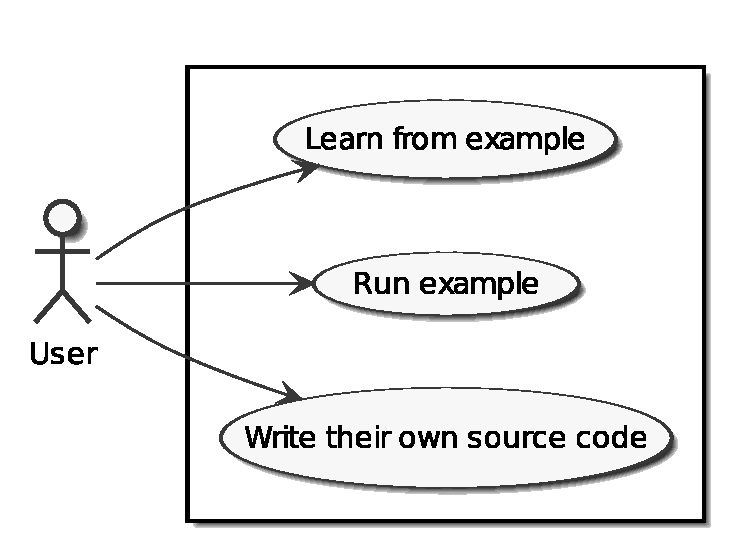
\includegraphics[width=.6\textwidth]{res/uml/use-cases-frontend.eps}%
        \caption{Il diagramma UML rappresenta i casi d'uso principali dell'interfaccia}%
        \label{fig:uml-use-case}
      \end{figure}

    \subsection{Requisiti non funzionali}\label{subsec:req:non-fun}
      Di seguito sono riportati i requisiti non funzionali che descrivono le proprietà non comportamentali che il sistema deve possedere.

      \begin{description}
        \item[Single-Page Application]
          Dal punto di vista dell'utente, l'applicativo web deve presentarsi come una singola pagina, permettendogli di gestire tutte le interazioni in un unico luogo.

        \item[Efficienza]
          L'esecuzione non deve appesantire il dispositivo client su cui esegue.
          Deve sfruttare in modo efficace le risorse messe a disposizione dalla macchina dell'utente.

        \item[Responsive, ma desktop-first]
          L'applicazione ha come destinazione d'uso il desktop, dunque non è necessaria un'interfaccia \emph{mobile-first}.
          È comunque necessario che il layout della pagina sia \emph{responsive}, ossia possa adattarsi a schermi di differenti misure e proporzioni.

        \item[Compatibilità con i browser]
          Il sistema dovrebbe essere supportato da quante più piattaforme browser possibile, con particolare attenzione a quelli più usati.
      \end{description}

  \section{Analisi dei requisiti e vincoli di fattibilità}

    L'applicazione web delineata dai requisiti non richiede strettamente la presenza di un server di appoggio:
    potenzialmente, come è stato visto anche nelle~\Cref{sec:web-architecture,subsec:online-ide}, le tecnologie sono sufficientemente mature
    da permettere la realizzazione di un ambiente in grado di modificare ed eseguire codice interamente all'interno della sandbox di un browser.
    In questo caso specifico, però, si è ritenuta imprescindibile la presenza di un esecutore remoto esterno.
    Infatti, come è stato più volte sottolineato nella~\Cref{part:background}, il linguaggio Protelis si appoggia alla piattaforma JVM per la sua esecuzione.
    Al momento della scrittura, l'unico supporto da parte delle tecnologie browser per Java ritenuto stabile era dato dal plugin per le Applet API\@.
    Tale plugin è stato deprecato da alcuni anni~\cite{jep289}, in concomitanza con il rilascio di Java 9;
    la quasi totalità dei browser ne ha ormai dismesso la compatibilità o lo farà a breve.
    Poiché il supporto ai browser più recenti e utilizzati è un requisito fondamentale, realizzare un esecutore per Protelis client-side è, al momento, impraticabile.

    Risulta dunque necessario distinguere i requisiti per il server esecutore dai requisiti dell'applicazione front-end che svolgerà il ruolo di client.

    \subsection{Requisiti del client}

      La componente client mantiene i requisiti funzionali già delineati ed analizzati nella~\Cref{subsec:req:fun}.
      Anche i requisiti non funzionali delineati nella~\Cref{subsec:req:non-fun} rimangono validi, ma viene aggiunto un ulteriore requisito.

      \begin{description}
        \item[Agnostico rispetto al backend]
          La rete dispositivi a cui si collega per l'esecuzione deve poter essere reale o virtuale senza che questo influenzi l'esperienza utente con il frontend.
          Le tecnologie utilizzate per l'implementazione del backend devono essere trasparenti al client.
      \end{description}

    \subsection{Requisiti del server}
      La componente server di questo progetto non deve interfacciarsi direttamente con l'utente, bensì fornire delle API generiche per l'esecuzione di codice Protelis proveniente dal client.

      Per questa entità, sono stati individuati i seguenti requisiti:

      \begin{description}
        \item[Esecuzione di codice Protelis]
          Il server deve poter eseguire codice Protelis ricevuto tramite le proprie API esposte in rete.
          In particolare, il server deve essere in grado di generare reti simulate di dispositivi su cui eseguire il codice \emph{on-demand}.

        \item[Supporto a più esecuzioni contemporanee]
          Il server deve permettere a più utenti di lavorare con il sistema contemporaneamente.
          In particolare, deve essere in grado di gestire più simulazioni, ciascuna distinta dalle altre e associata al client che l'ha richiesta.

        \item[Mantenimento della connessione]
          Il server deve essere in grado di mantenere una connessione bidirezionale stabile con ciascun client, in modo da permettere al client di ottenere aggiornamenti sullo stato dell'esecuzione.
      \end{description}

      Per quanto riguarda i requisiti non funzionali, sono state delineate le seguenti proprietà:

      \begin{description}
        \item[Scalabilità]
          Il sistema deve essere aperto alla possibilità di essere scalato efficacemente.
          In particolare, non è necessario che il prototipo sia in grado di scalare autonomamente, ma deve permettere l'introduzione di un eventuale orchestratore senza particolare difficoltà.

        \item[Protocollo di connessione efficiente]
          Il server deve esporre le proprie API tramite un protocollo efficiente dal punto di vista delle performance, non andando a limitare in modo sensibile la velocità con cui il frontend viene informato dei progressi dell'esecuzione.
          Inoltre, tali API dovrebbero permettere di sostituire lo standard di comunicazione senza la necessità di effettuare modifiche notevoli nel motore.

        \item[Compatibilità con i browser]
          Il protocollo di comunicazione utilizzato dal prototipo dovrebbe essere supportato da quante più piattaforme possibile (sia dal punto di vista dei browser che del server).
      \end{description}

  \section{Architettura logica}\label{sec:arch-logica}

  Una volta terminata l'analisi dei requisiti e del problema, è possibile delineare un'architettura logica che possa essere un punto di partenza per la fase di progettazione, descritta nel~\Cref{ch:project}.
  In particolare, la piattaforma da realizzare appare come un sistema software distribuito con struttura client-server composta da due entità principali:
  un'interfaccia Single-Page accessibile tramite browser permette all'utente di avere accesso alle API di un server che nascondono completamente tutta la complessità di configurazione della rete (reale o simulata), permettendo l'esecuzione del codice e il monitoring remoto.

    \chapter{Analisi del problema \& Progettazione}\label{ch:project}
  Una volta chiariti i requisiti del sistema, il passo successivo riguarda la progettazione dello stesso.
  In particolare, occorre delineare più nel dettaglio l'architettura di massima del sistema, per poi spostare l'attenzione su ciascuna entità interagente.

  % \section{Architettura del sistema}
  Come preventivato già in fase di analisi dei requisiti, il sistema vede la presenza di due principali entità:

  \begin{itemize}
    \item una pagina web che costituisce il client del sistema.
    \item un server di backend, che esegue su piattaforma JVM interfacciandosi con un esecutore di codice Protelis.
  \end{itemize}

  \begin{figure}[htbp]
    \centering
    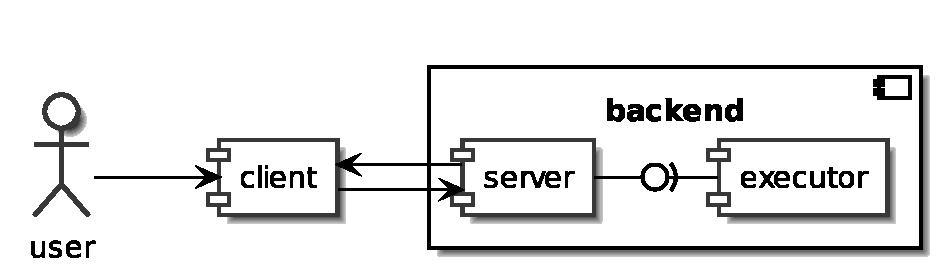
\includegraphics[width=.8\textwidth]{res/uml/architecture-design.eps}%
    \caption{Il diagramma UML riporta l'architettura di massima dei componenti del sistema}%
    \label{fig:architecture-design}
  \end{figure}

  Nelle \nameCrefs{sec:arch:client} successive di questo \nameCref{ch:project}, si intende analizzare più nel dettaglio questa struttura (della quale si ha una rappresentazione grafica in~\Cref{fig:architecture-design}),
  focalizzandosi sui dettagli di ciascun componente.

  \section{Design dell'applicazione}\label{sec:client-design}
    % TODO: inserire breve introduzione sulle GUI

    \subsection{Mockup dell'interfaccia}\label{subsec:mockup}
      Una volta chiariti i requisiti e le possibili fonti di ispirazione per la struttura della UI da realizzare, sono stati disegnati dei mockup che potessero rappresentare una linea guida
      per l'implementazione concreta dell'interfaccia.

      Come detto anche nella~\Cref{subsec:online-ide}, la struttura grafica dell'applicazione dovrebbe ispirarsi a quella di altri ambienti di sviluppo online,
      come ad esempio Overleaf (\Cref{fig:overleaf}).

      \begin{figure}[htbp]
        \centering
        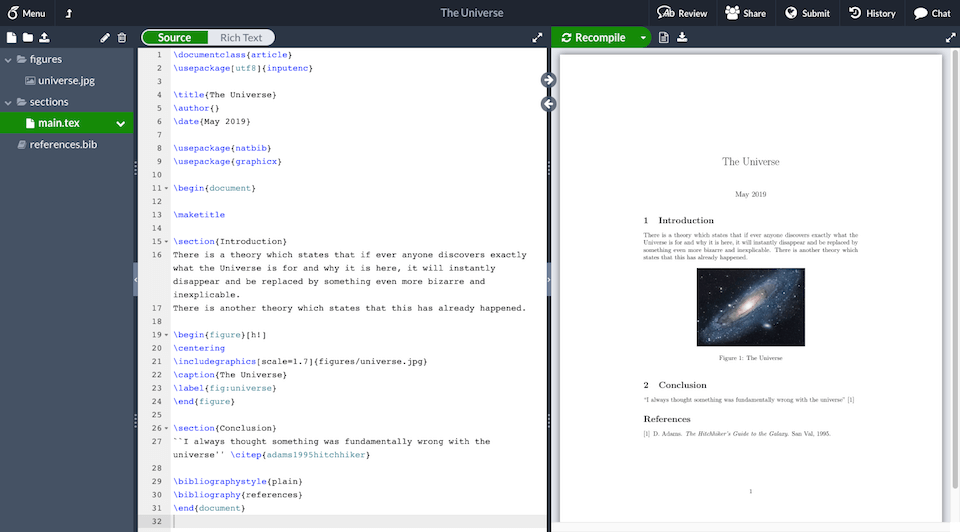
\includegraphics[width=.85\textwidth]{res/fig/overleaf.png}%
        \caption{Screenshot prelevato dalla pagina principale della web app Overleaf}%
        \label{fig:overleaf}
      \end{figure}

      Tali applicazioni hanno generalmente una struttura bipartita:
      nella parte sinistra è solitamente presente un editor che ricorda quello disponibile in diverse IDE desktop, mentre nella parte destra viene generalmente inserita una visualizzazione dell'output.
      Ad esempio, in Overleaf è possibile, alternativamente, visualizzare il log degli errori o il documento compilato.

      \begin{figure}[htbp]
        \centering
        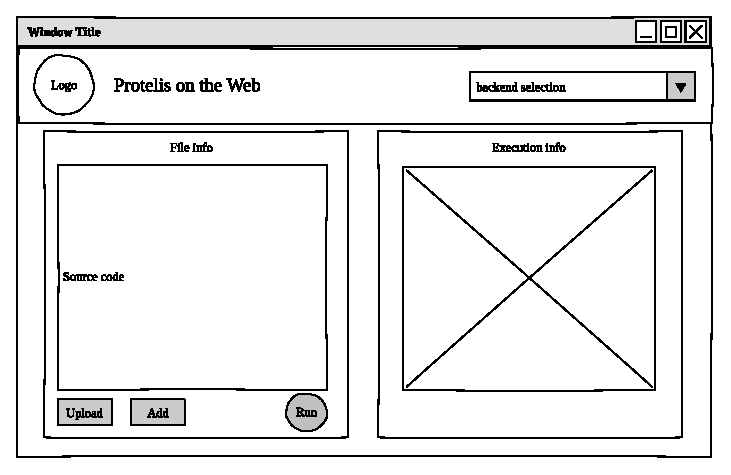
\includegraphics[width=.85\textwidth]{res/mockup/gui-actual.eps}%
        \caption{Mockup dell'interfaccia che dovrà presentare la pagina web}%
        \label{fig:mockup}
      \end{figure}

      Nel mockup finale, riportato in~\Cref{fig:mockup}, si è preso molto ispirazione da questo tipo di struttura.
      L'interfaccia dovrebbe infatti essere costituita dalle parti seguenti:

      \begin{itemize}
        \item
          Una \emph{barra superiore}, nella quale è riportato il nome e il logo del progetto, insieme a un selettore per il backend.
          Nei primi mockup, tale selettore era posizionato nella sezione principale della pagina, ma successivamente si è preferito spostarlo per sfruttare al meglio lo spazio a disposizione.
        \item
          Un \emph{blocco di sinistra}, che costituisce la parte con cui l'utente può interagire per lavorare sul codice.
          Il componente principale è appunto l'editor, un campo di testo avanzato che permette di visualizzare il codice Protelis di esempio e modificarlo.
          Sotto di esso sono presenti i bottoni di controllo per interagire con l'esecuzione.
        \item
          Un \emph{blocco di destra}, che ospita un canvas in cui l'esecuzione viene rappresentata.
          Al suo interno verranno visualizzati i nodi su cui il codice sta eseguendo.
          % In questa sezione, i componenti principali sono:
          % \begin{description}
          %   \item[Editor]
          %     Un campo di testo in cui visualizzare codice Protelis di esempio e modificarlo.
          %   \item[Play]
          %     Un bottone che permette di lanciare l'esecuzione del codice.
          %   % \item[Add]
          %   % TODO
          % \end{description}
      \end{itemize}

    \subsection{Design di riferimento}\label{subsec:material}
      Come è stato già sottolineato, l'applicazione vede come utilizzo principale quello dell'utente inesperto del linguaggio.
      L'interfaccia non deve essere solo semplice, ma anche moderna, gradevole e intuitiva.
      Era dunque necessario scegliere uno stile grafico familiare, moderno e facilmente adattabile a quella che sarebbe essere la nuova interfaccia che si stava progettando.

      Prendendo come esempio l'interfaccia di Overleaf (\Cref{fig:overleaf}), è possibile notare come il design di base abbia uno stile di tipo \emph{flat};
      si è deciso dunque di valutare tra i principali design possibili quali fosse più adeguato per la UX che si aveva intenzione di progettare.

      La scelta è infine ricaduta sul Material Design sviluppato da Google:
      dal suo annuncio nel giugno del 2014 al Google I/O 2014 Keynote esso è stato almeno parzialmente adottato in molte applicazioni web, mobile e desktop
      e ben si si presta all'implementazione di un'interfaccia semplice e minimale. % TODO eventualmente cita evoluzioni successive

      Per offrire un'esperienza coerente, si è deciso di utilizzare le icone e le direttive in merito a dimensioni e variazioni nella palette di colori fornite da Google\footnote{\url{https://material.io}}.
      Il colore base utilizzato per generare la palette è stato ricavato dall'icona ufficiale di Protelis. % TODO: cite logo

  \section{Architettura del client}\label{sec:arch:client}

    L'applicazione web che svolge il ruolo di client è a tutti gli effetti un'applicazione indipendente dotata di interfaccia grafica.
    % Sono stati valutati i numerosi pattern di modellazione documentati in letteratura e, alla fine,
    Sono numerosi i pattern di modellazione documentati in letteratura.
    % Molti di questi (genericamente definiti ``MV*'', ossia \emph{\emph{M}odel, \emph{V}iew} e qualsiasi cosa, generalmente \emph{Controller} o \emph{ViewModel}) tendono a distinguere entità che modellano il dominio
    % Tra tutti quelli considerati, si è scelto di adottare il \emph{pattern Flux} nella variazione chiamata \emph{pattern Redux}.
    La caratteristica maggiormente ricercata durante la progettazione è la reattività:
    il sistema dovrebbe aggiornarsi rapidamente sia quando l'utente lo richiede, interagendo via browser, sia quando il server manda un aggiornamento.

    % È stato dunque ritenuto necessario scegliere un approccio che ponesse al centro lo \emph{stato} del sistema, per poi scegliere, nella prossima fase, le tecnologie più adatte a reagire rapidamente alle sue variazioni.

    % Nelle \nameCrefs{subsec:state-manage} che seguono verranno prese in considerazione le scelte fatte decidendo il piano di lavoro.

    \subsection{Framework di sviluppo}\label{subsec:react}

      Sono disponibili numerosi framework per lo sviluppo di applicazioni web \emph{single-page}, ciascuna dei quali ottimizzata per determinati pattern di progettazione.
      Essendo un requisito la realizzazione di una SPA, la scelta di quale framework impiegare è fondamentale già in fase di progetto, in quando può notevolmente condizionare il piano di lavoro.

      Per l'implementazione di questo prototipo, è stato scelto il framework React, sviluppato da Facebook e compatibile, ufficialmente o meno, con numerosi linguaggi.
      Tecnicamente React, senza prendere in considerazione gli strumenti sviluppati intorno ad esso, sarebbe una libreria per la costruzione di pagine web reattive e \emph{data-driven};
      esso potrebbe essere considerato, riduttivamente, il \emph{view layer} dei pattern architetturali \emph{MV*} (\emph{Model View Anything}).
      React non è però vincolato al pattern MVC come AngularJS o a MVVM come Angular dalla versione 2 in poi.

      % In AngularJS, ogni vista è associata ad un controller, che si occupa della gestione dei dati e della loro visualizzazione.
      % La view è definita da un template, formata da elementi HTML, ed è compito dello sviluppatore associare la logica di controllo alla rappresentazione.

      La divisione principale che determina la struttura è quella tra \emph{componenti}.
      In React, un componente è un'astrazione che incapsula i dati, la loro manipolazione e la logica di rappresentazione e va a definire il più piccolo elemento costitutivo dell'applicazione.
      Esso rimuove la necessità del \emph{data-binding} tra modello e vista, tipico dei pattern MV*, e mantiene la logica applicativa all'interno di ciò a cui fa riferimento.

      Un componente definisce insomma cosa deve essere renderizzato;
      il sistema, autonomamente, determina in modo reattivo quando una delle dipendenze è cambiata e il componente può essere singolarmente ridisegnato.

      In questo modo, è possibile costruire applicazioni componendo tra loro questi elementi in una struttura simile a un albero, delegando la logica di gestione al motore di React, che se ne occuperà in modo efficiente.

      La progettazione dell'architettura deve dunque spostarsi sulla gestione dello stato.

      % React, come buona parte dei framework per lo sviluppo di applicazioni web, si basa sul concetto di \emph{componente}.
      %
      % Il successo di React deriva dalla visione innovativa della struttura di un'applicazione web.
      % React non presenta una separazione netta tra gli elementi di vista, presentazione e logica applicativa;

      % non esiste un controller, né data-binding

      % Anziché separare in modo deciso gli elementi di vista dal resto della logica applicativa (come invece accade tramite template e linguaggi di markup in Angular, ad esempio),

      % React incapsula
      % L'approccio tradizionale, adottato ad esempio da Angular, utilizza dei template realizzati tramite linguaggi di markup, dove la vista è realizzata tramite , sul quale vengono fatti

      % React nasce fondamentalmente come risposta al problema del \emph{change detection} che affligge.

      % start TODO
      % È stato dunque ritenuto necessario scegliere un approccio che ponesse al centro lo \emph{stato} del sistema, per poi scegliere, nella prossima fase, le tecnologie più adatte a reagire rapidamente alle sue variazioni.
      % end TODO

    \subsection{Pattern di gestione dello stato}\label{subsec:state-manage}
  Durante la fase di progettazione di un sistema software, è fondamentale definire la struttura con la quale le singole componenti saranno organizzate.

  Nel contesto applicativo di software orientati all'interazione con l'utente tramite interfaccia grafica, come ad esempio un'applicazione web,
  è spesso consigliato definire chiaramente la gestione dello stato e del flusso informativo, quando questi non sono imposti da eventuali framework utilizzati.

  Per esempio, come accennato nella~\Cref{subsec:react}, React prevede che la struttura dei componenti sia definita da un albero:
  lo stato di questi può fluire solo verso il basso, dunque si consiglia di mantenerlo il più alto possibile nella gerarchia;
  si parla infatti di ``\emph{state lift-up}''.
  Questo tipo di soluzione può risultare limitante in caso di un numero elevato di componenti, dunque sono stati elaborati pattern specifici per la gestione dello stato.

  \subsubsection{Flux architecture}
    Come alternativa al più classico \emph{Model-View-Controller} (MVC)~\cite{Reenskaug2003TheM},
    Facebook propone per le applicazioni React un nuovo pattern architetturale denominato Flux~\cite{10.1145/2742580.2742818}.
    Esso sottolinea la natura unidirezionale del flusso di dati in un'applicazione React (di qui il nome)
    e può essere di fatto considerato una variante del \emph{pattern Observer}~\cite{10.5555/186897} applicato all'architettura del sistema.

    \begin{figure}[htbp]
      \centering
      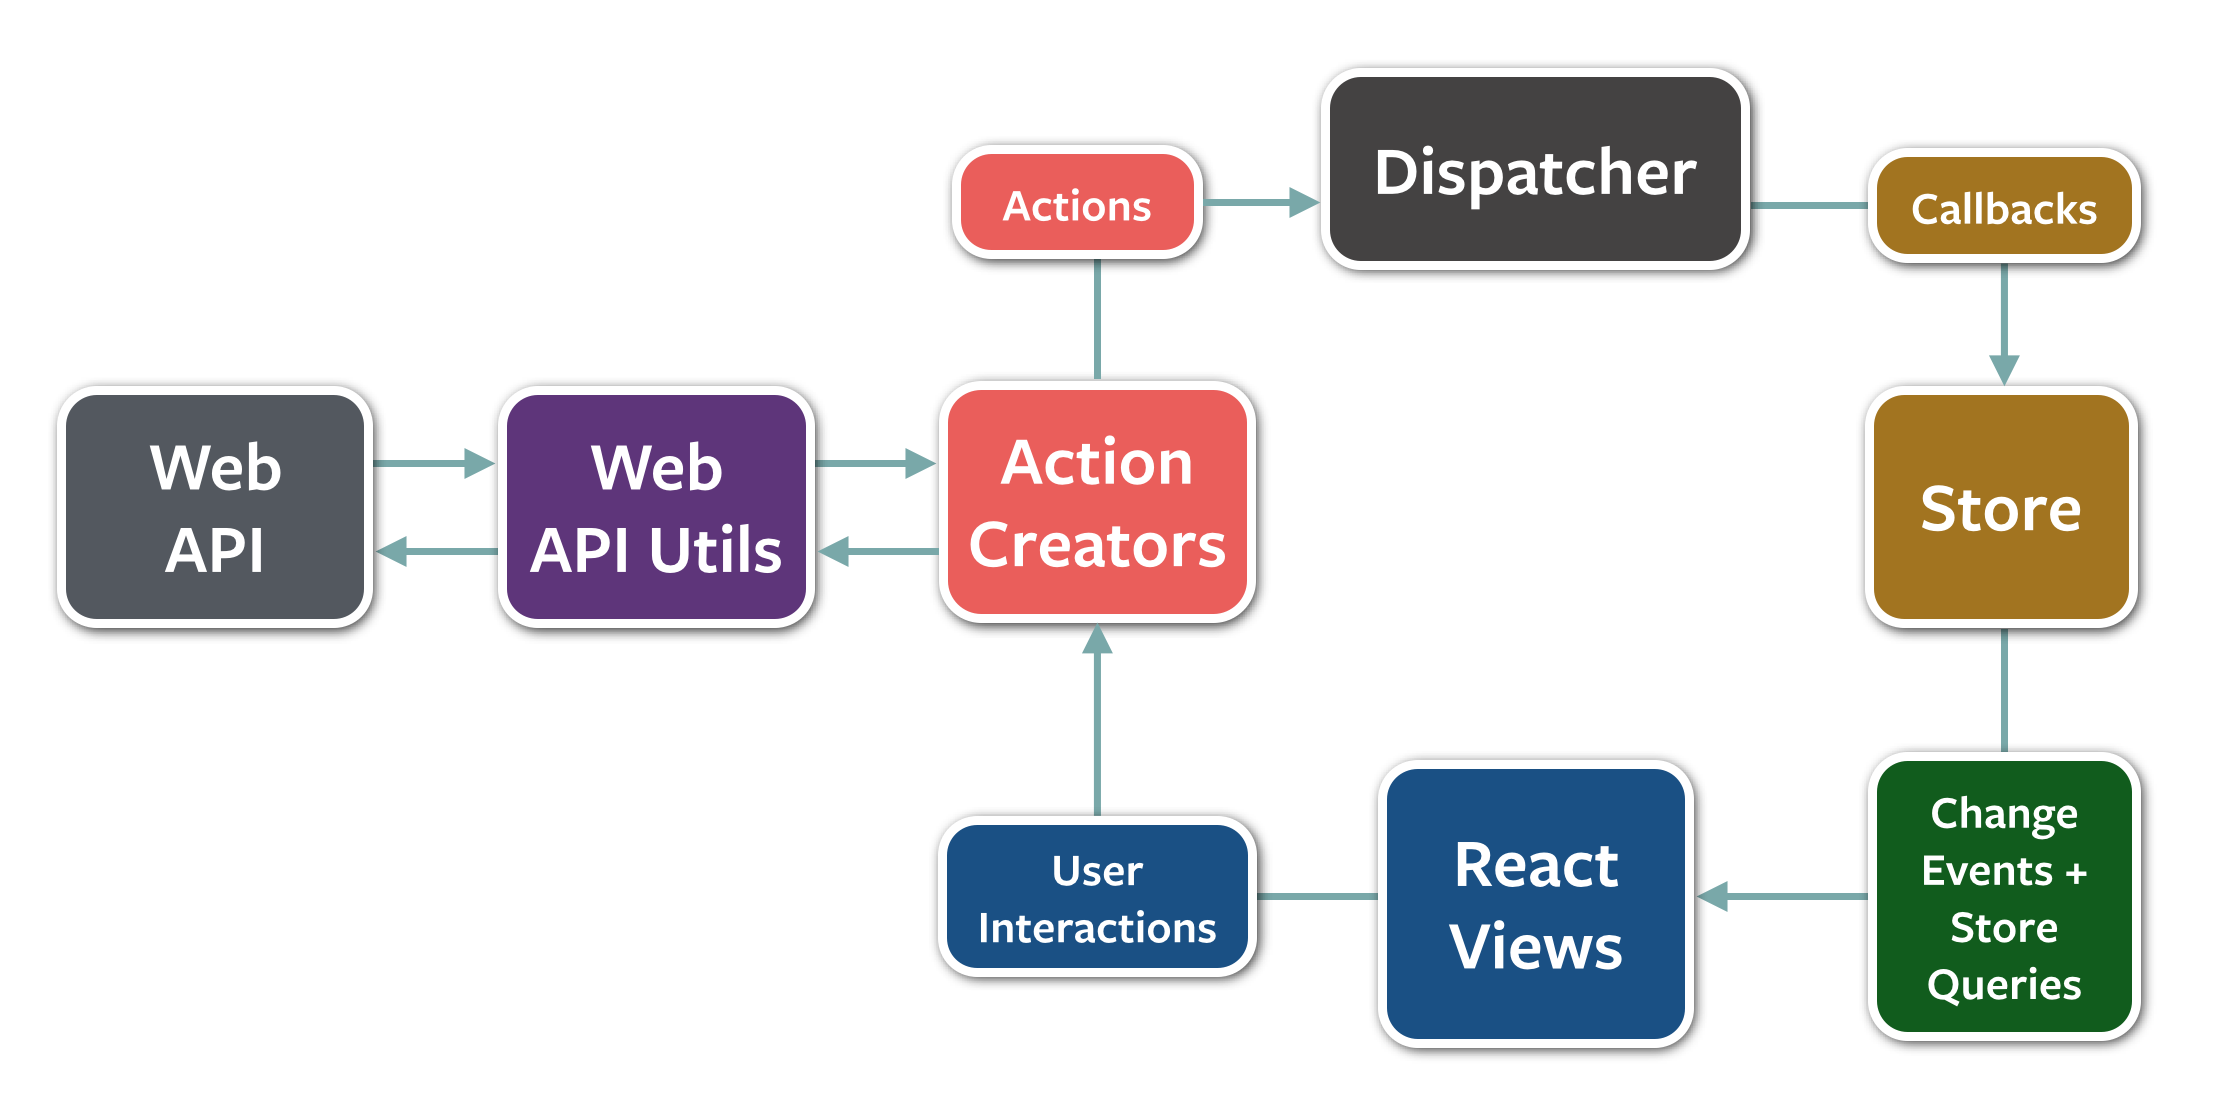
\includegraphics[width=.9\textwidth]{res/fig/flux-diagram-white-background.png}
      \caption[
        Rappresentazione del flusso unidirezionale dei dati in un'applicazione React con Flux.
      ]{
        Rappresentazione del flusso unidirezionale dei dati in un'applicazione React con Flux.
        Figura ripresa dalla documentazione ufficiale.
      }%
      \label{fig:flux}
    \end{figure}

    Come è possibile vedere in~\Cref{fig:flux}, la struttura è composta da quattro entità principali:
    \begin{description}
      \item[Store]
        Rappresenta il ``contenitore'' che incapsula lo \emph{stato} (del dominio applicativo e/o dell'interfaccia grafica).
        Ciascuno store agisce come \emph{single source of truth} (SSOT)
        e non permette di modificare direttamente i valori dello stato, ma solo tramite \emph{azioni} passate con un \emph{dispatcher}.
      \item[Dispatcher]
        Singolo oggetto che invia in broadcast come eventi le azioni agli store;
        gli store devono essere registrati per gli eventi che sono in grado di gestire all'avvio dell'applicazione.
      \item[View]
        Rappresenta la componente di interazione con l'utente;
        essa osserva gli store per aggiornarsi al variare dello stato e genera azioni sulla base delle richieste dell'utente.
        Sono possibili due tipi di view:
        \begin{description}
          \item[Presentation view] Non si collega né al dispatcher, né agli store, bensì comunica tramite \emph{proprietà} definite alla costruzione.
          \item[Container view] Si collega al dispatcher e/o agli store, reagendo agli eventi e/o generandoli.
        \end{description}
      \item[Action]
        Oggetto semplice e immutabile che contiene tutte le informazioni necessarie per modellare un'interazione con lo stato.
        Possono essere generate dalla view o da API web esterne, ma sempre attraverso un \emph{action creator}.
    \end{description}

    Il flusso informativo avviene dunque in una singola direzione e tramite \emph{callback}.
    Questo garantisce le seguenti proprietà:

    \begin{description}
      \item[Asincronismo]
        Il motore che interpreta JavaScript gestisce ciascuna callback eseguendola al ciclo successivo, non bloccando l'esecuzione attuale.
      \item[Consistenza di rappresentazione]
        Essendo ciascuno store centralizzato per l'intera applicazione, lo stato rappresentato dovrebbe essere univoco indipendentemente dalla pagina attuale.
      \item[Disaccoppiamento]
        Essendo lo store esterno ai componenti grafici, essi risultano maggiormente disaccoppiati rispetto al dominio e più riusabili.
      \item[Determinismo]
        Essendo lo stato aggiornabile solo tramite azioni, non si hanno effetti secondari e l'applicazione risulta più facile da rappresentare come una sequenza finita di stati, agevolando anche la fase di testing.
    \end{description}

  \subsubsection{Redux pattern}

    Il pattern Redux è una delle più popolari varianti del pattern Flux.

    Redux\footnote{\url{http://redux.js.org}} è il nome della libreria JavaScript per la gestione dello stato che per prima ne ha definito un'implementazione.
    Creata da Dan Abramov e Andrew Clark nel 2015 come implementazione alternativa a quella ufficiale del pattern Flux,
    essa combina idee provenienti dal pattern \emph{Command}~\cite{10.5555/186897} e dall'\emph{architettura Elm} teorizzata con l'omonimo linguaggio~\cite{czaplicki2012elm}:
    lo stato dell'applicazione è descritto da un singolo POJO (\emph{Plain Old JavaScript Object}) all'interno dello store e gli aggiornamenti avvengono tramite \emph{reducer}, funzioni pure di un'azione e dello stato corrente che generano un nuovo stato.

    \begin{figure}[htbp]
      \centering
      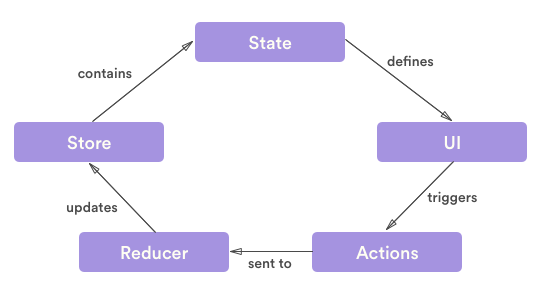
\includegraphics[width=.9\textwidth]{res/fig/redux-diagram.png}
      \caption[
        Rappresentazione del flusso unidirezionale dei dati in Redux.
      ]{
        Rappresentazione del flusso unidirezionale dei dati in Redux.

        Figura ripresa dalla documentazione ufficiale.
      }%
      \label{fig:redux}
    \end{figure}

    Secondo la documentazione ufficiale, la completa centralizzazione dello stato permette al sistema di essere completamente predicibile, permettendo il ``\emph{time-travel debug}'' tramite strumentazione integrata nel browser.
    Inoltre, il non essere strettamente legato a un framework di rappresentazione e la possibilità di caricare middleware lo rendono estremamente flessibile.

      Nel caso di questo progetto, tale soluzione è stata ritenuta ottimale per il tipo di architettura che si intende realizzare.

      Prendendo dunque in considerazione il mockup delineato alla~\Cref{subsec:mockup}, lo store sarebbe costituito dalle seguenti parti (dette \emph{slice}):

      \begin{description}
        \item[Editor]
          In \texttt{editorSlice} saranno inserite tutte le informazioni relative allo stato dei file.
          In particolare, è possibile definire al suo interno una struttura ad albero riguardante i file e lo stato di apertura degli stessi.
        \item[Esecuzione]
          In \texttt{execSlice} saranno invece inseriti i dati relativi all'esecuzione, come:
          \begin{itemize}
            \item lo stato della connessione,
            \item lo stato della simulazione,
            \item l'ID della simulazione,
            \item i dati dei nodi da rappresentare.
          \end{itemize}
      \end{description}

      \improvement[inline]{
        Mi piacerebbe aggiungere maggiori dettagli ``formali'', ad esempio graficamente con UML, ma non saprei come.

        Da quanto leggo online, non è esattamente il tipo di grafico adatto a questo tipo di pattern architetturale.
      }

  \section{Architettura del server}\label{sec:arch:server}

    Il server costituisce l'entità del sistema che si occupa dell'esecuzione del codice Protelis; è un esecutore remoto.

    Innanzitutto, è stato necessario chiarire se l'architettura dovesse essere monolitica o separata in microservizi.
    In tempi recenti, l'approccio a microservizi viene preferito a causa di diversi vantaggi:

    \begin{itemize}
      \item
        un sistema composto da microservizi indipendenti è più semplice da scalare,
        in quanto è possibile replicare ciascun servizio in modo indipendente dagli altri, a seconda delle esigenze.
      \item
        l'approccio a microservizi risulta generalmente più semplice da manutenere,
        in quanto disaccoppia i servizi tra loro, rendendo chiare le dipendenze condivise e permettendo lo sviluppo indipendente delle componenti.
      \item
        offrono un'integrazione migliore con orchestratori cloud e permettono di impiegare tecnologie di \emph{continuous deployment} (CD) in modo più efficiente.
    \end{itemize}

    Tali vantaggi sono però maggiormente evidenti quando le funzionalità che devono essere offerte sono \emph{tante}.
    Nel caso di questo progetto, di contro, il sistema deve essere in grado di gestire in modo efficiente un solo tipo di servizio, ossia l'esecuzione di codice su una rete simulata.

    In questo caso, dunque, è stato ritenuto più adeguato scegliere un'architettura monolitica, favorendo la semplicità di progettazione
    e delegando la gestione dello scaling al livello di piattaforma di deploy.

    \subsection{Pattern reactor}\label{subsec:reactor}

      Il giusto livello di reattività ed efficienza è stato trovato nell'approccio \emph{event-driven} con \emph{event-loop}.
      Tramite questo modello di concorrenza, denominato \emph{pattern Reactor}~\cite{Schmidt1995ReactorAO}, il server gestisce le richieste dei client attraverso una coda:
      uno o più cicli si occupano di gestire gli eventi nella coda in modo sincrono.
      In particolare, si è deciso di adottare il modello \emph{multi-reactor} fornito da Vert.x.

      \emph{Vert.x} è un framework applicativo event-driven che esegue su JVM (nonostante offra un supporto poliglotta a diversi linguaggi).
      Del modello architetturale messo a disposizione dal framework, è stato considerato interessante il concetto di \emph{Verticle}:
      esso è un'astrazione che incapsula un event-loop insieme al suo stato e interagisce tramite gli eventi provenienti da un event-bus.
      La documentazione\footnote{\url{https://vertx.io/docs/vertx-core/kotlin/\#_verticles}} % TODO: move to biblio
      specifica che l'approccio non può essere considerato pienamente \emph{ad attori}, bensì solo \emph{actor-like}.

      Per questo progetto, il modello è stato considerato adatto, in quanto in grado di garantire il giusto livello di astrazione e i criteri di reattività richiesti.

    \subsection{Verticle individuati}
      Il sistema progettato è composto da due componenti principali.

      \begin{itemize}
        \item
          Il primo, chiamato \texttt{BridgeVerticle}, è dedicato alla gestione delle API per la comunicazione da e verso l'esterno.
          % Esso si avvale dell'EventBus di Vert.x per comunicare con l'esterno
          In particolare, esso implementa il pattern \emph{bridge} relativamente alle connessioni verso l'esterno, trasformando le chiamate HTTP eseguite dai client in eventi espliciti dell'EventBus.
          % In questo modo, all'interno dell'applicazione, tutte le istanze dei verticle interessati possono essere
          Gestendo le comunicazioni con l'esterno, esso astrae l'intero processo di gestione del protocollo di comunicazione dalle altre componenti dell'applicazione.
        \item
          Il secondo è invece chiamato \texttt{AlchemistVerticle} e costituisce l'entità che si interfaccia con un motore di esecuzione esterno,
          come detto nell'architettura generale delineata all'inizio di questa fase di progettazione (\Cref{fig:architecture-design}).
          In particolare, per eseguire il codice si è scelto di utilizzare il simulatore Alchemist, che verrà analizzato più nel dettaglio nella~\Cref{subsec:alchemist}.
      \end{itemize}

      Oltre a questi, è stato anche progettato l'uso di un verticle principale \texttt{MainVerticle}, che viene lanciato dall'avviatore di Vert.x e che coordina l'avvio dei due verticle descritti sopra.

    \subsection{Simulatore scelto: Alchemist}\label{subsec:alchemist}
  Alchemist~\cite{alchemist-jos2013} è un meta-simulatore estendibile completamente \emph{open-source} che esegue su \engEmph{Java~Virtual~Machine}, nato all'interno dell'Università di Bologna.

  \subsubsection{Simulazione}\label{subsec:introAlchemist}
    In generale, una \emph{simulazione}~\cite{des3} è una riproduzione del modo di operare di un sistema o un processo del mondo reale nel tempo.
    L'imitazione del processo del mondo reale è detta \emph{modello};
    esso risulta essere una riproduzione più o meno semplificata del mondo reale, che viene aggiornata ad ogni passo di esecuzione della simulazione.

    Alchemist rientra nell'archetipo dei simulatori ad eventi discreti (DES)~\cite{des, des2}:
    gli eventi sono strettamente ordinati e vengono eseguiti uno alla volta, determinando il passare del tempo.
    L'idea dietro al progetto è quello di riuscire ad avere un framework di simulazione il più possibile generico, in grado di simulare sistemi di tipologia e complessità diverse, mantenendo le prestazioni dei simulatori non generici (come ad esempio quelli impiegati in ambito chimico~\cite{gillespie1976}).

    Per perseguire questo obiettivo, la progettazione dell'algoritmo è partita dallo studio del lavoro di Gillespie del 1977~\cite{gillespie1977} e di altri scienziati nell'ambito della simulazione chimica.
    Nonostante siano presenti algoritmi in grado di eseguire un numero di reazioni addirittura in tempo costante, la scelta dell'algoritmo è infine ricaduta su una versione migliorata dell'algoritmo SSA di Gillespie, il Next Reaction Method~\cite{nextReactionMethod} di Gibson e Bruck:
    ad ogni passo di simulazione, esso è in grado di selezionare la reazione successiva in tempo costante e richiede un tempo logaritmico per aggiornare le strutture dati interne al termine dell'esecuzione dell'evento.

  \subsubsection{Astrazioni e modello}\label{subsec:modello}

    Il modello di astrazione di Alchemist è ispirato dal lavoro della comunità scientifica nell'ambito dei simulatori a scopo di ricerca chimica e ne riprende dunque la nomenclatura.
    Le entità (visibili in \Cref{fig:alchemist:model}) su cui lavora sono le seguenti:

    \begin{description}
      \item[Molecola]\label{itm:mol}
        Una \emph{molecola} rappresenta il nome assegnato ad un particolare dato all'interno di un \emph{nodo}, del quale ne astrae parte dello stato.

        Un parallelismo con la programmazione imperativa vedrebbe la \emph{molecola} come un'astrazione del nome di una variabile.

      \item[Concentrazione]\label{itm:conc}
        La \emph{concentrazione} di una \emph{molecola} è il valore associato alla proprietà rappresentata dalla \emph{molecola}.

        Mantenendo il parallelismo con la programmazione imperativa, la \emph{concentrazione} rappresenterebbe il valore della variabile.

        \begin{figure}[tbp] % h rimosso per posizionare correttamente la footnote
          \centering
          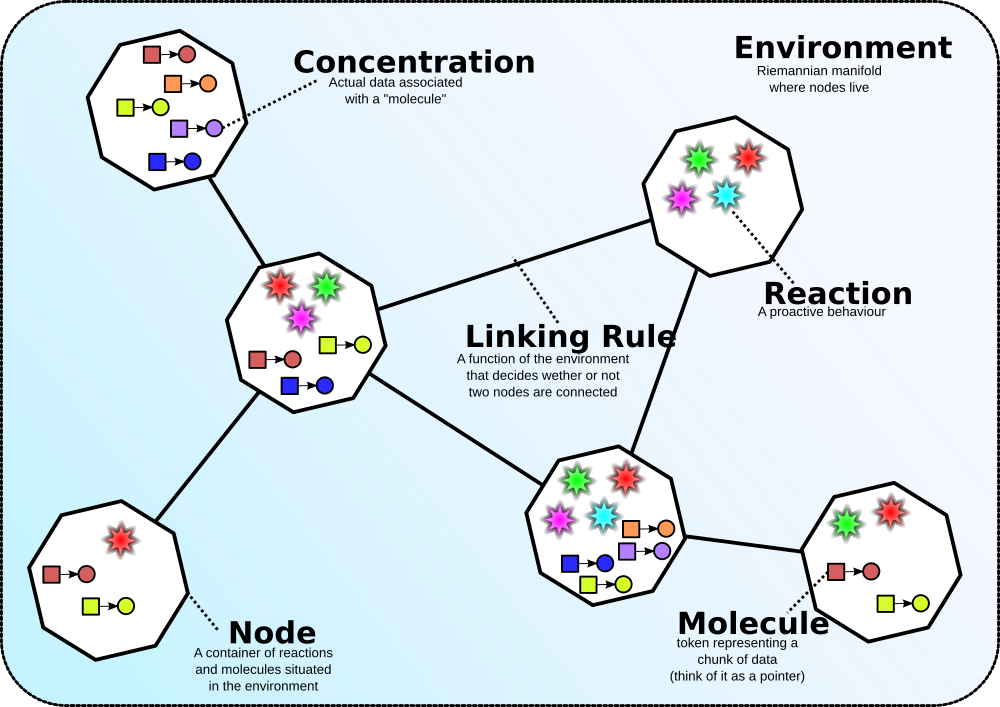
\includegraphics[width=.85\textwidth]{res/fig/alchemist_model.png}
          \caption[%
            Rappresentazione grafica delle diverse entità di Alchemist.
          ]{%
            Rappresentazione grafica delle diverse entità di Alchemist.\\
            Figura ripresa dal sito ufficiale\protect\footnotemark.
          }%
          \label{fig:alchemist:model}
        \end{figure}
        \footnotetext{\url{http://alchemistsimulator.github.io}}

      \item[Nodo]\label{itm:node}
        Il \emph{nodo} è un contenitore di \emph{molecole} e \emph{reazioni} che risiede all'interno di un \emph{ambiente} e che astrae una singola entità.

      \item[Ambiente]\label{itm:env}
        L'\emph{ambiente} è l'astrazione che rappresenta lo spazio nella simulazione ed è l'entità che contiene i \emph{nodi}.

        Esso è in grado di fornire informazioni in merito alla posizione dei \emph{nodi} nello spazio, alla distanza tra loro e al loro vicinato;
        opzionalmente, l'\emph{ambiente} può offrire il supporto allo spostamento dei \emph{nodi}.

      \item[Regola di collegamento]\label{itm:linkr}
        La \emph{regola di collegamento} è una funzione dello stato dell'\emph{ambiente} che associa ad ogni \emph{nodo} un \emph{vicinato}.

      \item[Vicinato]\label{itm:neigh}
        Un \emph{vicinato} è un'entità costituita da un \emph{nodo} detto ``centro'' e da un insieme di altri \emph{nodi} (i ``vicini'').

        L'astrazione dovrebbe avere un'accezione il più possibile generale e flessibile, in modo da poter modellare qualsiasi tipo di legame di vicinato, non solo spaziale.

        \begin{figure}[htbp]
          \centering
          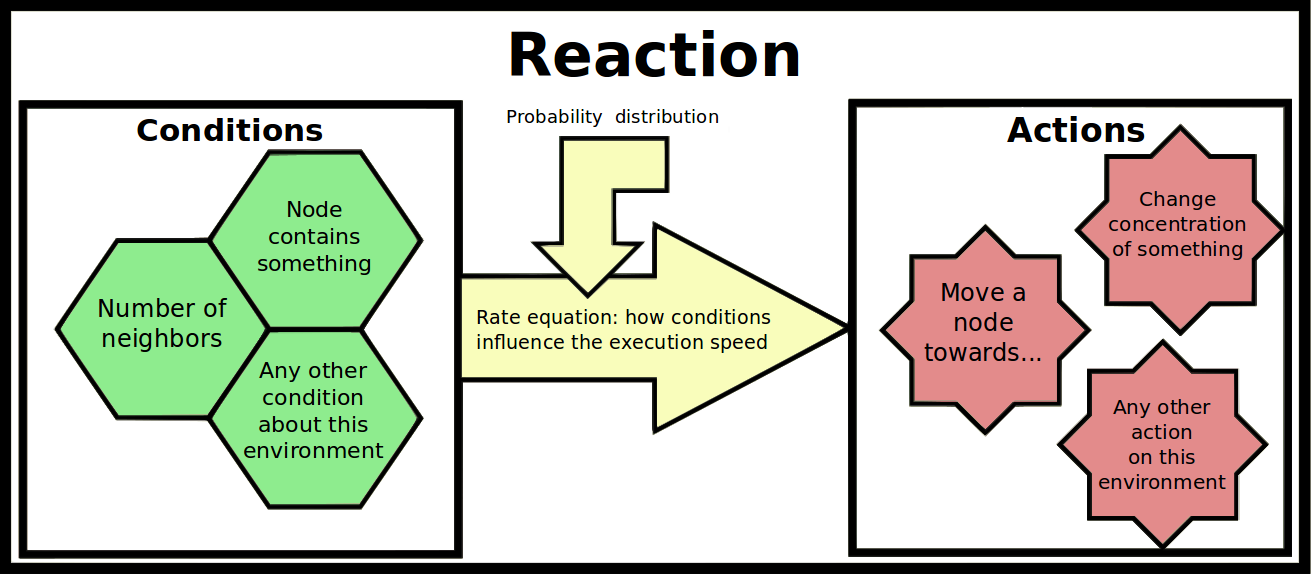
\includegraphics[width=.85\textwidth]{res/fig/alchemist_reaction.png}
          \caption{Rappresentazione grafica della \emph{Reazione}.}%
          \label{fig:alchemist:reaction}
        \end{figure}

      \item[Reazione]\label{itm:react}
        Il concetto di \emph{reazione} è da considerarsi molto più elaborato di quello utilizzato in chimica:
        in questo caso, si può considerare come un insieme di \emph{condizioni} sullo stato del sistema, che qualora dovessero risultare vere innescherebbero l'esecuzione di un insieme di \emph{azioni}.

        Una \emph{reazione} (di cui si ha una rappresentazione grafica in~\Cref{fig:alchemist:reaction}) è dunque un qualsiasi evento che può cambiare lo stato dell'\emph{ambiente} e si compone di un insieme di \emph{condizioni}, una o più \emph{azioni} e una distribuzione temporale.

        La frequenza di accadimento può dipendere da:
        \begin{itemize}
            \item Un tasso statico;
            \item Il valore di ciascuna \emph{condizione};
            \item Una equazione che combina il tasso statico e il valore delle \emph{condizioni}, restituendo un ``tasso istantaneo'';
            \item Una distribuzione temporale.
        \end{itemize}

        Ogni \emph{nodo} è costituito da un insieme (anche vuoto) di \emph{reazioni}.

      \item[Condizione]\label{itm:cond}
        Una \emph{condizione} è una funzione che associa un valore numerico e un valore booleano allo stato corrente di un \emph{ambiente}.

      \item[Azione]\label{itm:act}
        Un'\emph{azione} è una procedura che provoca una modifica allo stato dell'\emph{ambiente}.

    \end{description}

    Per quanto la terminologia sia ripresa dalla chimica, il meta-modello del simulatore è estendibile, adottando interpretazioni più o meno lasche dei termini ``molecola'' e ``concentrazione''.
    In particolare, in Alchemist esiste il concetto di \emph{incarnazione}, che definisce l'istanza concreta del meta-modello, delineando le modalità con le quali le astrazioni vengono implementate.

  \subsubsection{Incarnazione Protelis}

    Alchemist fornisce l'implementazione di diverse incarnazioni;
    per lo scopo di questa tesi, ci si propone di utilizzare l'incarnazione Protelis.
    In essa, la molecola identifica il nome di un sensore, mentre la sua concentrazione è il valore misurato.

    Attraverso la configurazione di Alchemist, è possibile definire il posizionamento dei nodi e le modalità di collegamento, nonché la presenza di specifiche molecole.
    In questo modo, è possibile definire una molecola che conterrà il codice Protelis che ciascun nodo deve eseguire;
    il sistema può così caricare dinamicamente il codice ottenendo la relativa concentrazione.
    Un esempio di configurazione è riportato in~\Cref{app:yaml}.


  \section{Interazioni}\label{sec:arch:interaction}

    \unsure[inline]{
      Ho deciso di descrivere le interazioni in una sezione dedicata, anziché separarle nelle sezioni del client e del server.

      È accettabile? O sarebbe meglio spezzare?
    }

    Una volta analizzato il comportamento delle due entità in gioco, è necessario delineare anche la loro interazione remota.

    \subsection{Scelta del modello di comunicazione e del protocollo}

      % Innanzitutto, è stato necessario chiarire quale tipo di comunicazione è necessario instaurare.
      Come detto nella \Cref{subsec:reactor}, per la progettazione del server di backend si è scelto di utilizzare un modello a event-loop multipli comunicanti tramite EventBus;
      inoltre, anche il pattern di gestione dello stato scelto per il funzionamento del client (\Cref{subsec:state-manage}) è event-driven.
      È risultato dunque naturale strutturare anche la comunicazione tra client e server utilizzando un modello a eventi.

      In particolare, l'EventBus di Vert.x supporta l'utilizzo di \emph{bridge} per la comunicazione remota attraverso numerosi protocolli.
      Tra questi, quello identificato come più adatto è \emph{SockJS}\@.

      SockJS è un protocollo pensato per realizzare una comunicazione \emph{WebSocket-like} sul maggior numero di piattaforme possibili.
      Esso gestisce in modo autonomo la verifica del supporto del protocollo WebSocket~\cite{Melnikov2011} da parte del client e del server, migrando su \emph{polling} tramite HTTP standard in caso assenza.
      Tramite un protocollo di questo tipo, è possibile realizzare un canale di comunicazione bidirezionale veloce, adatto per il trasferimento di un elevato numero di eventi come nel caso di questo progetto di tesi.

      Dunque, il \texttt{BridgeVerticle} esporrà tramite API (al percorso ``\texttt{/eventbus}'' relativamente all'\emph{host} principale) l'accesso all'EventBus per i messaggi previsti.
      L'applicazione web si dovrà connettere attraverso un client generando azioni sullo store interno.

    \subsection{Comportamento}

      Una volta chiarite le modalità di trasferimento delle informazioni, viene progettato il comportamento che permette al sistema di essere reattivo.
      In~\Cref{fig:event:vertx} viene rappresentata la sequenza di operazioni svolte dal server sulla base degli eventi inoltrati sull'EventBus di Vert.x;
      in~\Cref{fig:event:redux}, invece, il diagramma UML riassume la sequenza di azioni che permutano lo stato di Redux con il procedere dell'esecuzione.
      Di seguito, invece, sono riassunti i passaggi nel loro complesso.

      \begin{itemize}
        \item
          il primo passo è instaurare la connessione.
          La pressione di un bottone genera un'azione sullo store che abilita la connessione SockJS verso il backend.
          L'utente viene notificato del risultato dell'operazione attraverso la generazione, da parte del sistema, di azioni con le relative permutazioni dello stato.
          % In questo modo, l'interfaccia permette all'utente di trovare un backend valido e di collegarcisi attraverso socket.
        \item
          una volta che il codice Protelis è pronto per essere lanciato, l'utente utilizzerà il bottone dedicato per eseguirlo.
          Questo causa la creazione di un'azione di richiesta di upload del codice;
          esso è già presente nello store, dal quale viene prelevato e inoltrato tramite socket al server.
        \item
          il verticle riceve l'evento tramite EventBus;
          procede dunque costruendo un simulatore, al quale viene assegnato un identificativo univoco e un componente osservatore.
          Dopodiché, tramite EventBus viene inviato l'identificativo.
        \item
          il client riceve questo ID tramite socket e un'azione di Redux viene generata.
          La vista viene aggiornata di conseguenza, informando l'utente dell'avvenuta configurazione e dell'imminente avvio dell'esecuzione.
        \item
          quando il motore di simulazione esegue uno step, il componente osservatore viene notificato.
          Viene dunque generato un evento sul bus degli eventi diretto verso l'esterno, su un indirizzo legato all'identificativo iniziale e alla tipologia di variazione avvenuta nella simulazione (step iniziale, \emph{round} d'esecuzione, terminazione).
        \item
          quando l'esecuzione viene terminata sul simulatore, il client viene notificato dell'evento nello stesso modo con cui ha ricevuto i vari aggiornamenti.
          Sul server, l'ID verrà classificato come terminato e il simulatore potrà essere riutilizzato o distrutto a seconda delle necessità.
      \end{itemize}

      \begin{figure}[htbp]
        \centering
        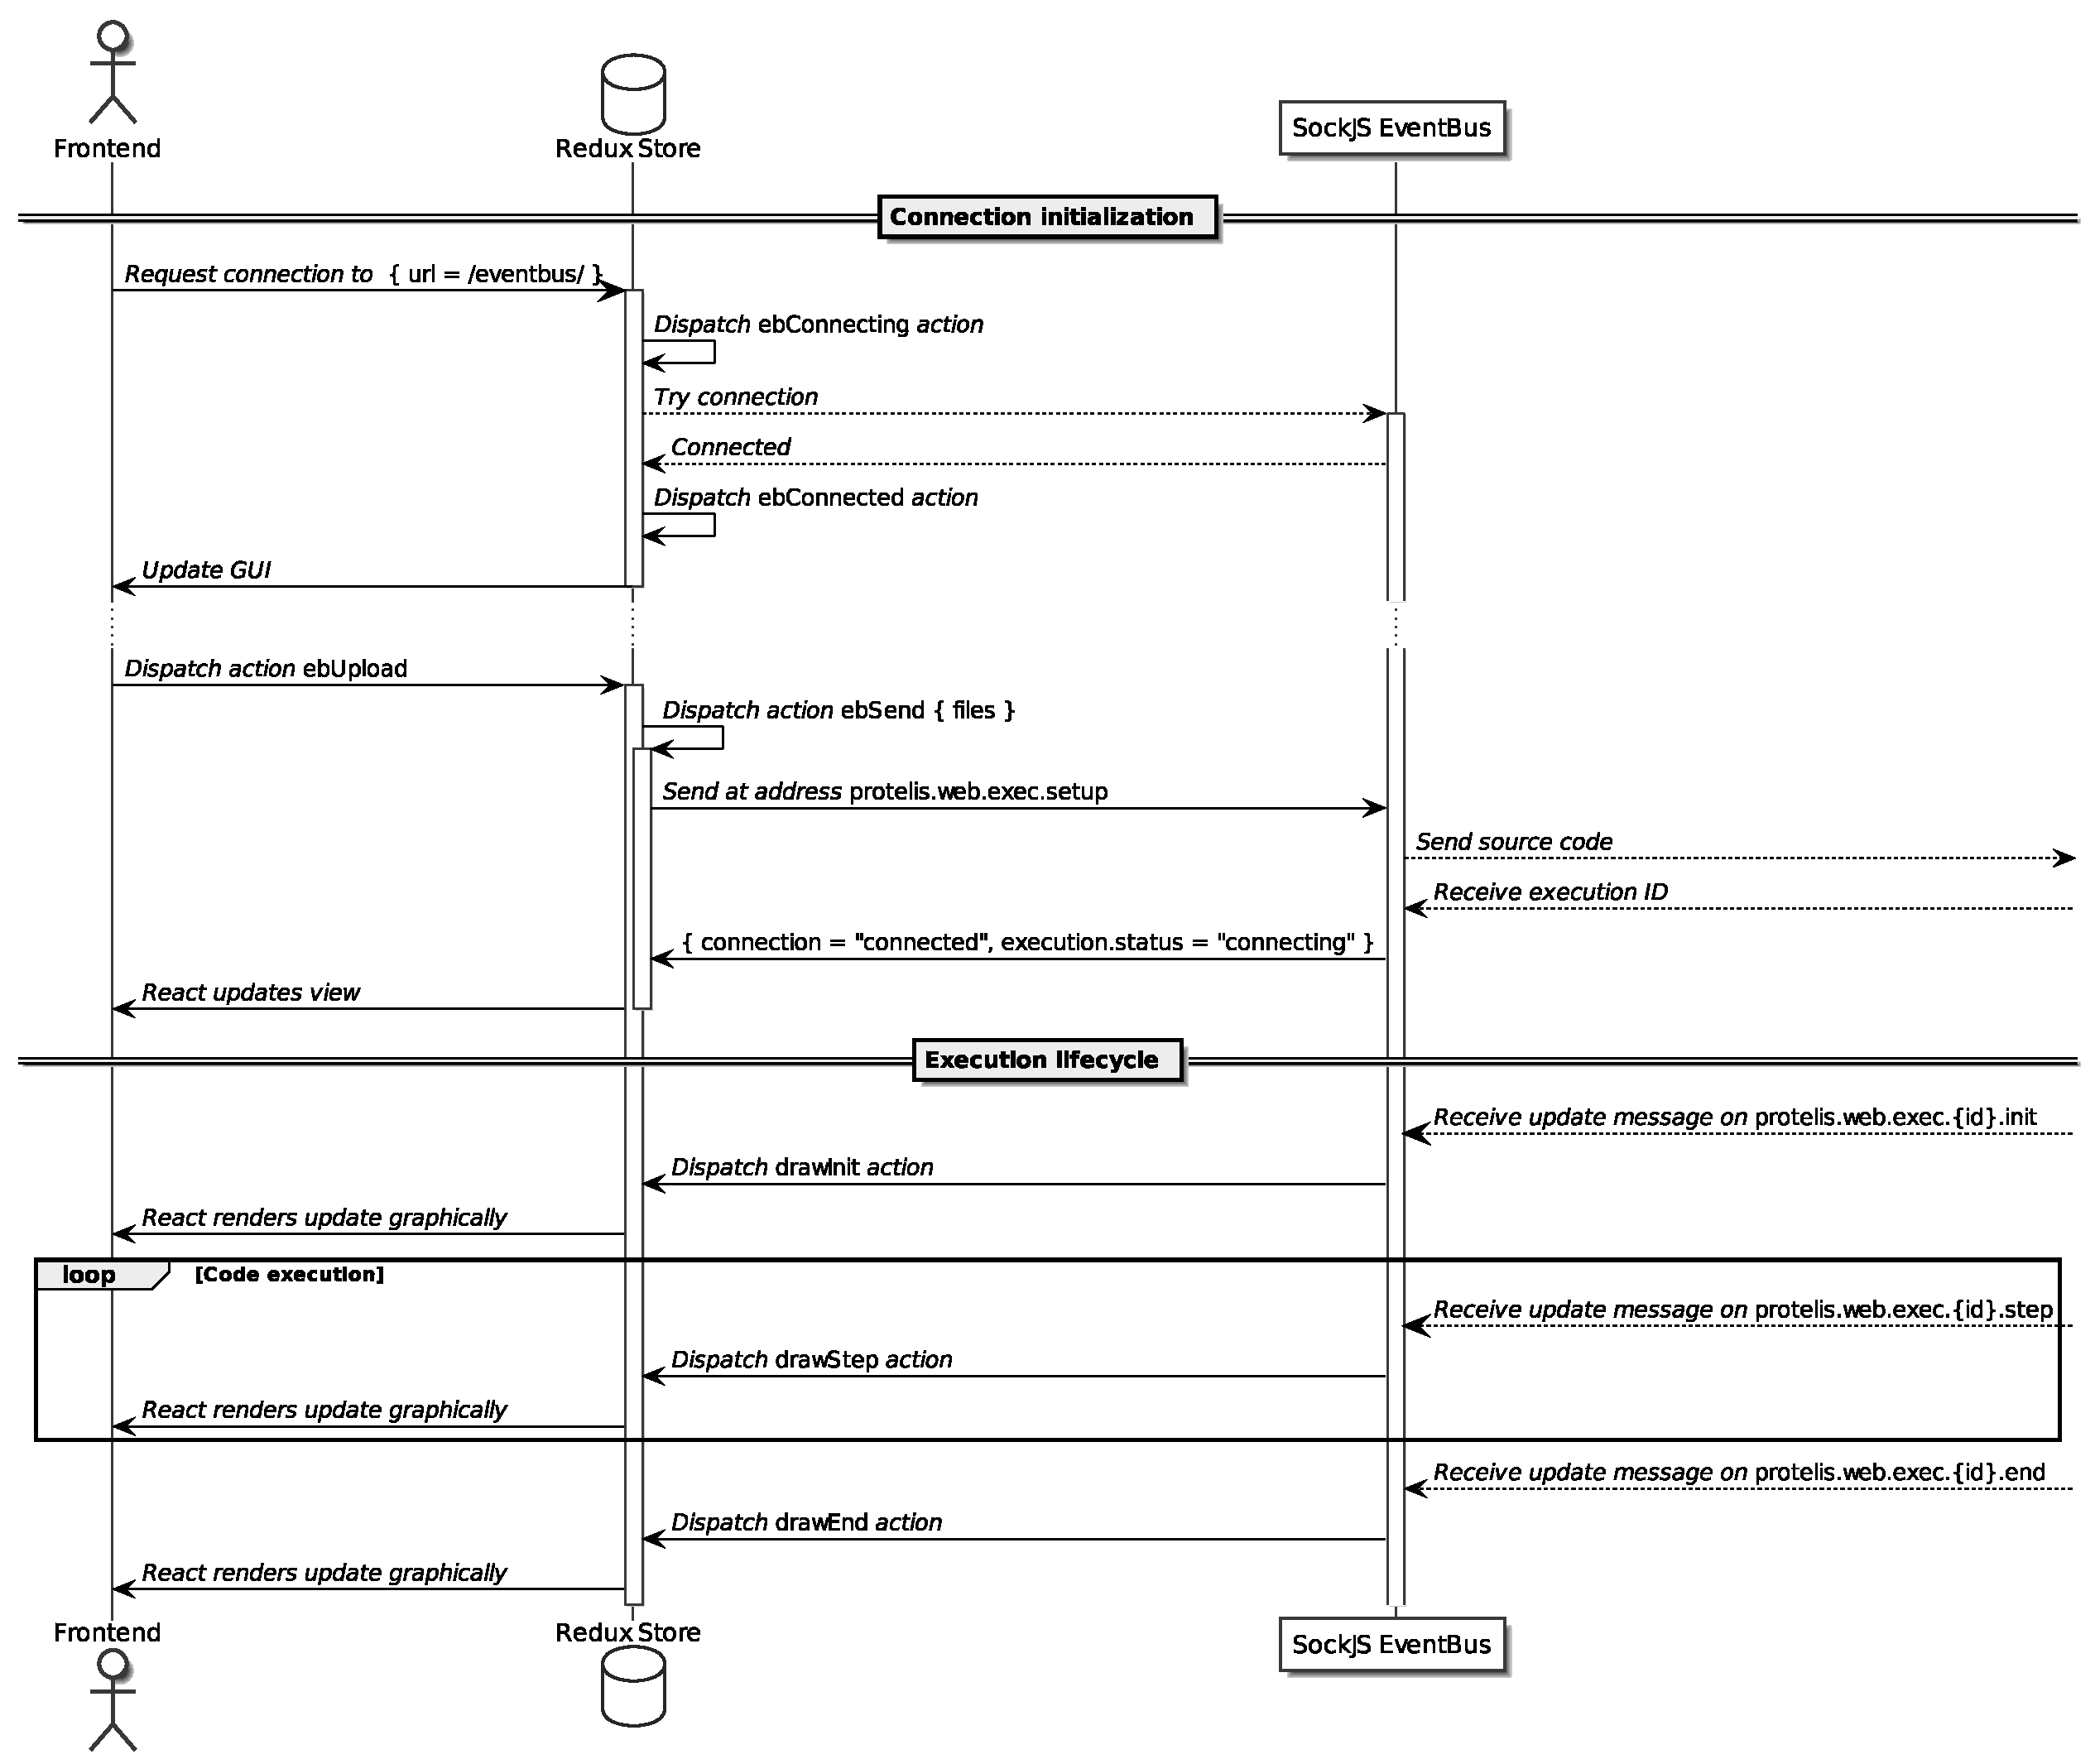
\includegraphics[width=.9\textwidth]{res/uml/redux-eventbus.eps}%
        \caption{Diagramma UML di sequenza rappresentante il flusso delle azioni sullo store di Redux.}%
        \label{fig:event:redux}
      \end{figure}

      \begin{figure}[htbp]
        \centering
        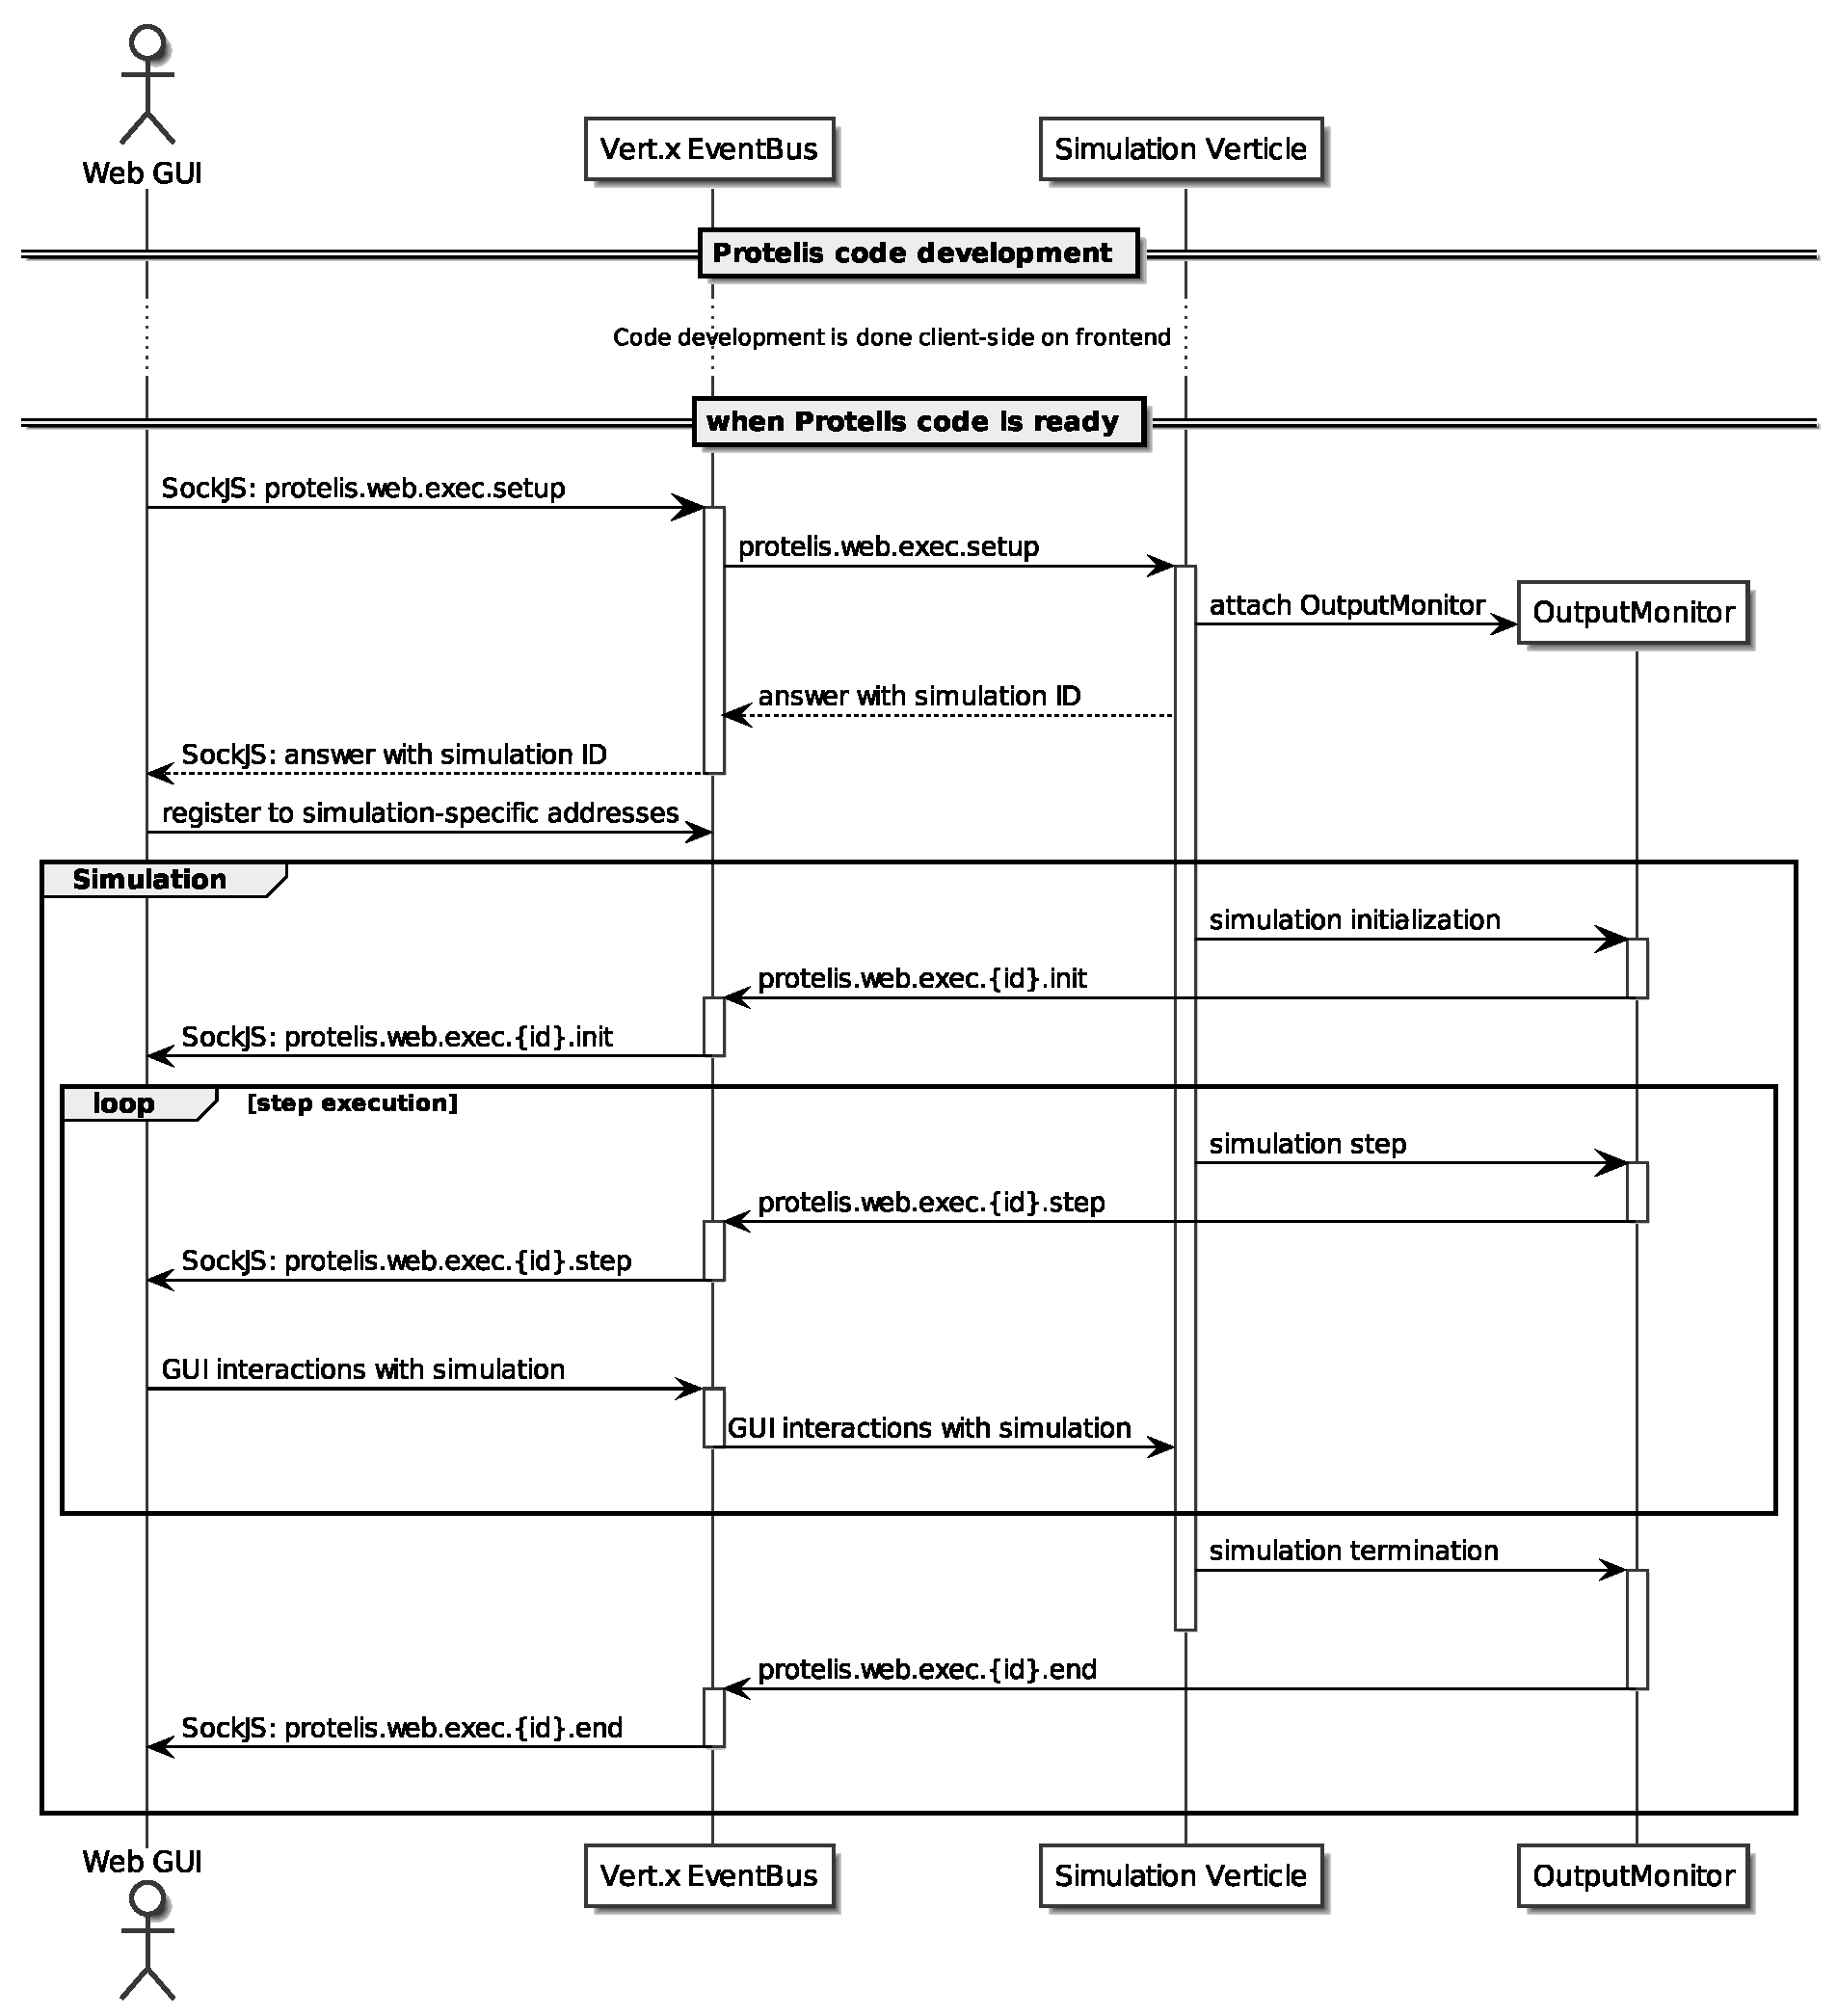
\includegraphics[width=.9\textwidth]{res/uml/data-flow.eps}%
        \caption{Diagramma UML di sequenza che rappresenta la gestione degli eventi sul bus di Vert.x.}%
        \label{fig:event:vertx}
      \end{figure}

    \chapter{Implementazione}\label{ch:implementation}
  In questo \nameCref{ch:implementation} sono esposti tutti i dettagli legati al processo di sviluppo e all'implementazione.
  In particolare, verranno motivate le scelte tecnologiche che in fase di progettazione non erano state considerate rilevanti.
  Inoltre, verranno analizzati alcuni dettagli implementativi ritenuti importanti alla descrizione del funzionamento del progetto.

  \section{Tecnologie utilizzate}

  \subsection{Linguaggi di programmazione}
    Il sistema è stato realizzato in due differenti linguaggi. Di seguito sono espresse le motivazioni della scelta di ciascuno di essi.

    \subsubsection{Linguaggio per il backend: Kotlin}

      Per la realizzazione del backend, come è stato specificato nel~\Cref{ch:requirements}, era necessario l'impiego di un linguaggio in grado di eseguire su piattaforma JVM\@.
      Il framework scelto, Vert.x, è presentato come poliglotta (supporta Java, JavaScript, Groovy, Ruby, Ceylon, Scala e Kotlin), non vincolando dunque la scelta.

      Si è deciso di procedere con Kotlin per le seguenti motivazioni:

      \begin{description}
        \item[Brevità ed espressività]
          Kotlin si presenta come molto meno verboso di Java, supportando un maggior numero di costrutti che permettono di ridurre il codice ``\emph{boilerplate}''.

        \item[Sicurezza]
          Una delle funzionalità che è stata pubblicizzata maggiormente alla presentazione di Kotlin è la \emph{null-safety}.
          Kotlin permette di evitare le comuni eccezioni di tipo \texttt{NullPointerException} gestendo il valore \texttt{null} in modo maggiormente chiaro tramite notazione opzionale e controllo da parte del compilatore.

        \item[Interoperabilità]
          Kotlin nasce per essere affiancato a Java e sostituirlo gradualmente.
          Risulta dunque intercompatibile con quasi qualsiasi piattaforma o libreria sia pensata per Java, non limitando eventualmente l'affiancamento futuro ad un altro linguaggio.

          Inoltre, il compilatore di Kotlin supporta diversi altri target, come browser, piattaforme mobile e binario nativo X86 e ARM, lasciando dunque aperte ulteriori possibilità di espansione future.

        \item[Approccio funzionale]
          Kotlin è principalmente un linguaggio orientato agli oggetti, ma supporta molti costrutti tipici della programmazione funzionale, come espressioni \emph{lambda}, \emph{function types} e le funzioni di ordine superiore.

        % \item[Performance]
          % Kotlin  pone  alcuni  miglioramenti  prestazionali nelle funzioni di ordine superiore e lambda, dimostrandosi più ottimizzato e veloce nei confronti di Java

        \item[Pragmatismo]
          Kotlin presenta, secondo la documentazione, l'intento di essere ``pragmatico'', ossia focalizzato sull'esperienza d'uso dello sviluppatore.
          Esso offre una buona integrazione con gli strumenti esistenti, sia per la costruzione (come Gradle e Maven) che per lo sviluppo (come Eclipse, Visual Studio e gli IDE di JetBrains).
      \end{description}

      Vert.x offre inoltre una estensione della propria libreria \emph{core} per sfruttare al meglio la sintassi di Kotlin.

    \subsubsection{Linguaggio per il frontend: TypeScript}\label{subsub:ts}
      Per la realizzazione del frontend era necessario l'impiego di un linguaggio in grado di eseguire su browser, quindi che fornisse come target di compilazione JavaScript o WebAssembly.
      A differenza del backend, il framework scelto, React, vincolava la scelta a un numero limitato di linguaggi in grado di generare codice JS\@.
      In particolare, sono stati presi in considerazione i quattro linguaggi introdotti nella~\Cref{sec:lang}, ma si è preferito impiegare TypeScript per i seguenti motivi:

      \begin{description}
        \item[Supporto ufficiale]
          Per quanto React venga presentato anche nella documentazione ufficiale come non strettamente dipendente dal linguaggio, il supporto disponibile per ciascuno di questi può essere differente.
          In particolare, Facebook, dichiara il supporto diretto solo per JavaScript e TypeScript;
          linguaggi come Kotlin, Scala, Reason e F\# sono dichiaratamente compatibili, ma la loro integrazione non è una priorità per la società.

          Kotlin (attraverso JetBrains) e Scala (attraverso il progetto Scala.js) offrono un supporto comunitario sufficiente, ma comunque non comparabile a quello offerto da Facebook e Microsoft.\unsure{Dovrei citare statistici da GitHub per sostenere questa posizione?}

        \item[Type Checking]
          JavaScript supporta unicamente la tipizzazione dinamica.
          Se questo aspetto da un lato aggiunge flessibilità al linguaggio, dall'altro aumenta la possibilità di bug e situazioni non previste.
          TypeScript offre un sistema di tipi completo e flessibile, che permette di definire una struttura chiara e flessibile, rendendo il processo di sviluppo più sicuro.

          Facebook supporta ufficialmente anche Flow e la libreria \texttt{prop-types} come alternativa all'utilizzo di un diverso linguaggio.
          Flow non offre però la medesima espressività di TypeScript e non può vantare un supporto altrettanto vasto da parte della comunità per la tipizzazione delle librerie JavaScript.
          La libreria \texttt{prop-types} invece offre un controllo dei tipi unicamente a tempo di esecuzione, richiedendo la definizione del tipo atteso manualmente.
          Questo non permette di adottare un approccio ``\emph{fail-fast}'' come quello vantato da TypeScript.

        \item[Integrazione con gli IDE]
          La possibilità di avere informazione sui tipi a livello di compilatore permettono a IDE come Visual Studio Code e WebStorm di essere molto più precisi ad evidenziare codice errato rispetto all'approccio basato su commenti di JavaScript.

        \item[Estensione della sintassi JSX e TSX]
          Una delle maggiori particolarità del framework React è la sintassi \emph{JSX}\@.
          L'acronimo sta per \emph{\emph{J}ava\emph{S}cript e\emph{X}tension} e identifica un particolare zucchero sintattico non presente in JavaScript ``standard''.
          Esso permette la definizione di ``\texttt{element}'', ossia di componenti direttamente rappresentabili, attraverso una sintassi dichiarativa di markup che ricorda HTML\@. \unsure{Dovrei inserire uno snippet di confronto?}

          Essendo in React la logica rappresentativa strettamente legata agli elementi non grafici del componente, essere in grado di distinguere in modo chiaro i \emph{concetti}\improvement{Non sono sicuro di aver espresso correttamente in italiano ``separation of concerns'', che sarebbe da traduzione separazione di interessi}
          all'interno dello stesso componente e file senza doversi affidare a markup esterno è un vantaggio notevole.

          TypeScript supporta questa estensione della sintassi, denominandola \emph{TSX}.

      \end{description}

      L'unica alternativa ritenuta valida al posto di TypeScript era Kotlin.
      L'impiego di Kotlin per tutta l'applicazione sarebbe stato infatti molto interessante per utilizzare un unico linguaggio in tutto il sistema, migliorando l'integrazione e il supporto a dipendenze condivise.

      Purtroppo, per quanto JetBrains supporti ufficialmente React per Kotlin/JS, l'integrazione all'inizio dei lavori di questa tesi era ancora troppo instabile per un uso reale.
      Si sono riscontrati problemi con lo strumento di generazione dei \emph{wrapper} per i tipi\unsure{Dovrei citare la issue GitHub che avevamo creato?} e l'output del compilatore genera codice JS datato e pesante.
      Fintanto che la versione 1.4 di Kotlin non sarà rilasciata in pianta stabile, si ritiene che il linguaggio non sia ancora pronto per un uso frontend su browser.

  \subsection{Strumenti per lo sviluppo e il controllo del software}\label{subec:quality}
    Per gestire le dipendenze in sistemi moderni, l'uso di applicazioni per la \emph{build-automation} dotati di risoluzione delle dipendenze è l'approccio più comune.

    L'utilizzo di strumenti che controllino la qualità del codice e diano la possibilità di testarlo in modo immediato è invece fondamentale per la realizzazione di un sistema complesso.
    Essi permettono infatti di revisionare il codice in modo sistematico, così da evitare errori che a volte possono verificarsi, senza bisogno che il programma venga realmente eseguito:
    analizzano il codice sorgente per individuare potenziali bug e spesso indicano possibili miglioramenti e ottimizzazioni.
    % Spesso tali strumenti vengono integrati nel processo di costruzione del codice.

    Essendo le due componenti basate su ecosistemi completamente diversi, verranno trattate separatamente.

    \subsubsection{Backend}

      Il progetto di backend utilizza Gradle per la risoluzione delle dipendenze, la costruzione del software e la verifica della qualità.
      \emph{Gradle} è un sistema per l'automazione dello sviluppo, nato per includere tutte le caratteristiche provenienti da Apache Ant, Maven e Ivy attraverso la definizione di \engEmph{buildscript} originariamente in Groovy e più recentemente anche in Kotlin.
      Pensato per i linguaggi che compilano per JVM, questo sistema permette di scaricare le dipendenze da diversi repository Maven durante la fase di compilazione.
      Nello script di costruzione sono stati utilizzati i seguenti plugin:

      \begin{description}
        \item[Gradle Shadow]
          Il plugin, sviluppato da John Engelman, permette la generazione di ``shadow jar'', ossia pacchetti jar contenenti anche tutte le dipendenze oltre al codice compilato.

        \item[Vert.x Gradle Plugin]
          Il plugin, sviluppato da Julien Ponge e adottato quasi ufficialmente dai manutentori del progetto Vert.x, fornisce una configurazione del progetto ottimizzata per progetti Vert.x.
          Rende possibile il lancio dei verticle in modo indipendente e con la ricompilazione automatica, molto comodo in sede di sviluppo e debug.

        \item[Kotlin]
          Il plugin, realizzato in modo ufficiale da JetBrains, configura Gradle per la compilazione di codice Kotlin e la configurazione delle opzioni per la generazione del bytecode.

          Per motivi di compatibilità con il simulatore Alchemist, è stata scelta come versione target del bytecode Java 11.

        \item[Ktlint Gradle]
          Il plugin, realizzato da Jonathan Leitschuh, è un wrapper dello strumento di analisi statica di codice Kotlin \emph{ktlint}, realizzato da Pinterest.
          Si è scelto di utilizzare ktlint anziché \emph{detekt}, altro strumento simile, in quanto non richiede una configurazione personalizzata, bensì impone un insieme standard di regole, comunemente studiate e accettate dalla community.

        \item[refreshVersions]\unsure{Qui la minuscola è \emph{voluta}, in quanto il plugin non ha un nome formale. Dovrei metterlo comunque maiuscolo come gli altri?}
          Il plugin, sviluppato da Jean-Michel Fayard, permette una migliore gestione delle dipendenze automatizzandone gli aggiornamenti.

        \item[JUnit]
          \emph{JUnit} è uno dei più noti framework di unit testing per Java e linguaggi derivati.
          Il plugin, integrato ufficialmente in Gradle, permette l'esecuzione di test automatizzati con tale framework.

          In questo progetto è stata utilizzata la versione 5 di JUnit, utilizzando il motore di esecuzione \emph{jupiter}.
        \item[JaCoCo]
          \emph{JaCoCo} è uno strumento per la misura della copertura del codice da parte dei test realizzati.
          Si integra con JUnit ed è pensato per Java e linguaggi derivati.
          Il plugin, integrato ufficialmente in Gradle, offre una dettagliata configurazione e permette la generazione di report in diversi formati.
      \end{description}

      Per lo sviluppo del codice è stato utilizzato l'ambiente di sviluppo integrato \emph{JetBrains Intellij IDEA} in versione \emph{Ultimate 2019.3.3}.
      Si è scelto questo rispetto ad altri IDE (come ad esempio Eclipse) in quanto in grado di offrire un'integrazione migliore con Gradle e Kotlin.

    \subsubsection{Frontend}

      Il progetto frontend è un modulo Node.js generato tramite lo strumento ufficiale \texttt{create-react-app} fornito da Facebook.
      Si seguito vengono riportate tutte le tecnologie utilizzate durante lo sviluppo:

      \begin{description}
        \item[Yarn]
          Come \emph{package manager} per la gestione delle dipendenze è stato scelto \emph{Yarn} anziché NPM\@.
          Esso, oltre a essere la scelta consigliata da React, presenta alcuni vantaggi rispetto alla controparte:
          \begin{itemize}
            \item La cartella delle dipendenze risulta generalmente più compatta in quanto utilizza collegamenti simbolici per le dipendenze condivise dai moduli JS risolti.
            \item La velocità di risoluzione delle dipendenze è generalmente più elevata, in quanto sfrutta una strategia di cache più efficiente.
          \end{itemize}

        \item[react-scripts]
          Lo strumento \texttt{create-react-app} astrae la complessità di configurazione di un progetto attraverso l'utilizzo di \texttt{react-scripts}.
          Essi incapsulano strumenti quali WebPack, Babel, ESLint e Jest, mettendo a disposizione semplici script che si appoggiano alle configurazioni ufficiali di riferimento per:
          \begin{inparaitem}
            \item compilazione,
            \item esecuzione,
            \item verifica
          \end{inparaitem}
          del codice realizzato.

        \item[ESLint \& stile Airbnb]
          \emph{ESLint} è uno strumento estendibile per l'analisi statica del codice, che supporta nativamente JavaScript e TypeScript.
          Il pacchetto \texttt{react-scripts} fornisce una configurazione minimale, ma è consigliato di adottare uno stile (insieme di regole) tra quelli più famosi.
          In questo caso è stato scelto quello fornito da Airbnb. % , in quanto uno dei più popolari.

        \item[Jest]
          \emph{Jest} è un framework di test per JavaScript sviluppato da Facebook che fornisce tutti gli strumenti per la scrittura e l'esecuzione dei test e per la raccolta della loro copertura sul codice.
      \end{description}

      Per lo sviluppo del codice è stato utilizzato l'ambiente di sviluppo integrato \emph{JetBrains WebStorm} in versione \emph{2019.3.3}.

  \subsection{Controllo di versione e CI/CD}
    Il controllo di versione utilizzato per questo progetto è affidato al DVCS (\emph{\emph{D}istributed \emph{V}ersion \emph{C}ontrol \emph{S}ystem}) Git, utilizzato con flusso di lavoro di tipo \emph{Git flow}.

    % Il codice è disponibile su GitHub nei repository seguenti:
    % \begin{itemize}
    %     \item \url{https://github.com/NiccoMlt/Protelis-Web} per il backend;
    %     \item \url{https://github.com/NiccoMlt/protelis-web-frontend} per il frontend.
    % \end{itemize}

    Il codice è disponibile su GitHub nei repository Protelis-Web\footnote{\url{https://github.com/NiccoMlt/Protelis-Web}}\improvement{Dovrei creare un DOI con Zotero?}
    e protelis-web-frontend\footnote{\url{https://github.com/NiccoMlt/protelis-web-frontend}}.
    % Si è preferito utilizzare due depositi separati anziché raggruppare in ciò che viene generalmente definito \emph{monorepo} poiché le differenti ...

    Attraverso GitHub sono allacciate ai repository le soluzioni di \emph{continuous integration} (CI):

    \begin{description}
      \item[Travis CI]
        \emph{Travis CI} è un sistema di integrazione continua distribuito, utilizzato per la compilazione e il test di progetti caricati su repository GitHub.
        Ad ogni operazione di push sul repository, il codice viene testato su tutte le maggiori piattaforme (Linux, Windows, MacOS) e le differenti versioni degli SDK (NodeJS LTS, AdoptOpenJDK con OpenJDK HotSpot e AdoptOpenJDK con Eclipse OpenJ9).
        Viene inoltre fatto un controllo sulla qualità del codice.

      \item[Codecov]
        Tramite \emph{Codecov} vengono raccolti i report di copertura del codice generati da JaCoCo e Jest, permettendo la visualizzazione online di grafici di dettaglio.
        Al termine di ogni esecuzione di una \emph{pipeline} in Travis CI, i report sulla piattaforma di riferimento vengono pubblicati qui.

      \item[Codacy]
        \emph{Codacy} è uno strumento online per l'automazione della \emph{code review} che aggrega diversi strumenti di analisi del codice per numerosi linguaggi, generando report dettagliati.
        Ad ogni operazione di push sul repository, il codice viene verificato.
    \end{description}

  \subsection{Deployment}
    Vert.x non si basa su \emph{servlet} e può essere eseguito su qualsiasi piattaforma permetta il lancio di un jar, senza la necessità di un hosting specifico per Java EE\@.

    Per motivi di test, il server è in esecuzione su due differenti piattaforme:

    \begin{itemize}
      \item
        Al termine della pipeline di Travis CI per il branch principale, l'eseguibile viene automaticamente caricato e lanciato su Heroku.

        \emph{Heroku} è un servizio online di tipo PaaS (\emph{\emph{P}latform as a \emph{S}ervice}) di proprietà di SalesForce e compatibile con diversi linguaggi.
        Informazioni sulla VM utilizzata non sono disponibili.
      \item
        Per performance migliori, viene utilizzato anche un server fornito dall'Università di Bologna.
        Su di esso viene effettuato il deploy tramite SSH avvalendosi del \texttt{docker-engine} in esecuzione all'interno di Linux.

        \emph{Docker} è uno strumento per la virtualizzazione a livello di sistema operativo (\emph{container}) molto utilizzato per la pacchettizzazione delle applicazioni.
        Il Dockerfile per la costruzione dell'immagine utilizzata, basato su AdoptOpenJDK con Eclipse OpenJ9, è allegato a questo documento in~\Cref{app:docker}.
    \end{itemize}

    Il client React è compilato come un bundle JavaScript importato da una pagina HTML\@.
    Esso non viene servito dal server Vert.x, bensì attraverso la piattaforma di hosting statico \emph{ZEIT Now}, che ne esegue il \emph{continuous deployment} direttamente da GitHub.

    % Per quanto riguarda il \emph{continuous deployment} (CD), sarà trattato nel dettaglio nella sottosezione successiva.

      % \subsection{Librerie esterne}
  % \subsection{Strumenti di sviluppo}
  %   In questa sezione verranno presentati tutti gli strumenti utilizzati per sviluppare il codice del sistema,
  %   descrivendone la loro utilità e il loro impiego.

  %   \subsubsection{Ambiente di sviluppo}
  %     Un IDE, o \emph{Integrated Development Environment} è un software che aiuta i programmatori nello sviluppo del codice sorgente di un software.\unsure{Non sono sicuro che questa parte sia necessaria}
  %     Esso mette a disposizione tutta una serie di strumenti e funzionalità utili per lo sviluppo e il debugging.
  %     Solitamente uno strumento di questo tipo mette a disposizione un editor di testo, un compilatore o un interprete (o entrambi) e un debugger.

  %     Per lo sviluppo di questo sistema sono stati utilizzati due IDE forniti da JetBrains: Intellij IDEA e WebStorm.
  %     In particolare,


  \section{Dettagli implementativi: Frontend}

    Per l'implementazione dei componenti di base del frontend, si è fatto largo uso della libreria Material-UI\@.
    Essa mette a disposizione una grande quantità di componenti React di base (come elementi per il layout e elementi di controllo) aderenti al design Material scelto in fase di progettazione.
    Inoltre, tramite la libreria è stato possibile definire un tema specifico per il progetto Protelis on Web nelle due varianti chiara e scura, caricate a seconda delle preferenze del browser dell'utente.

    \begin{figure}[htbp]
      \centering
      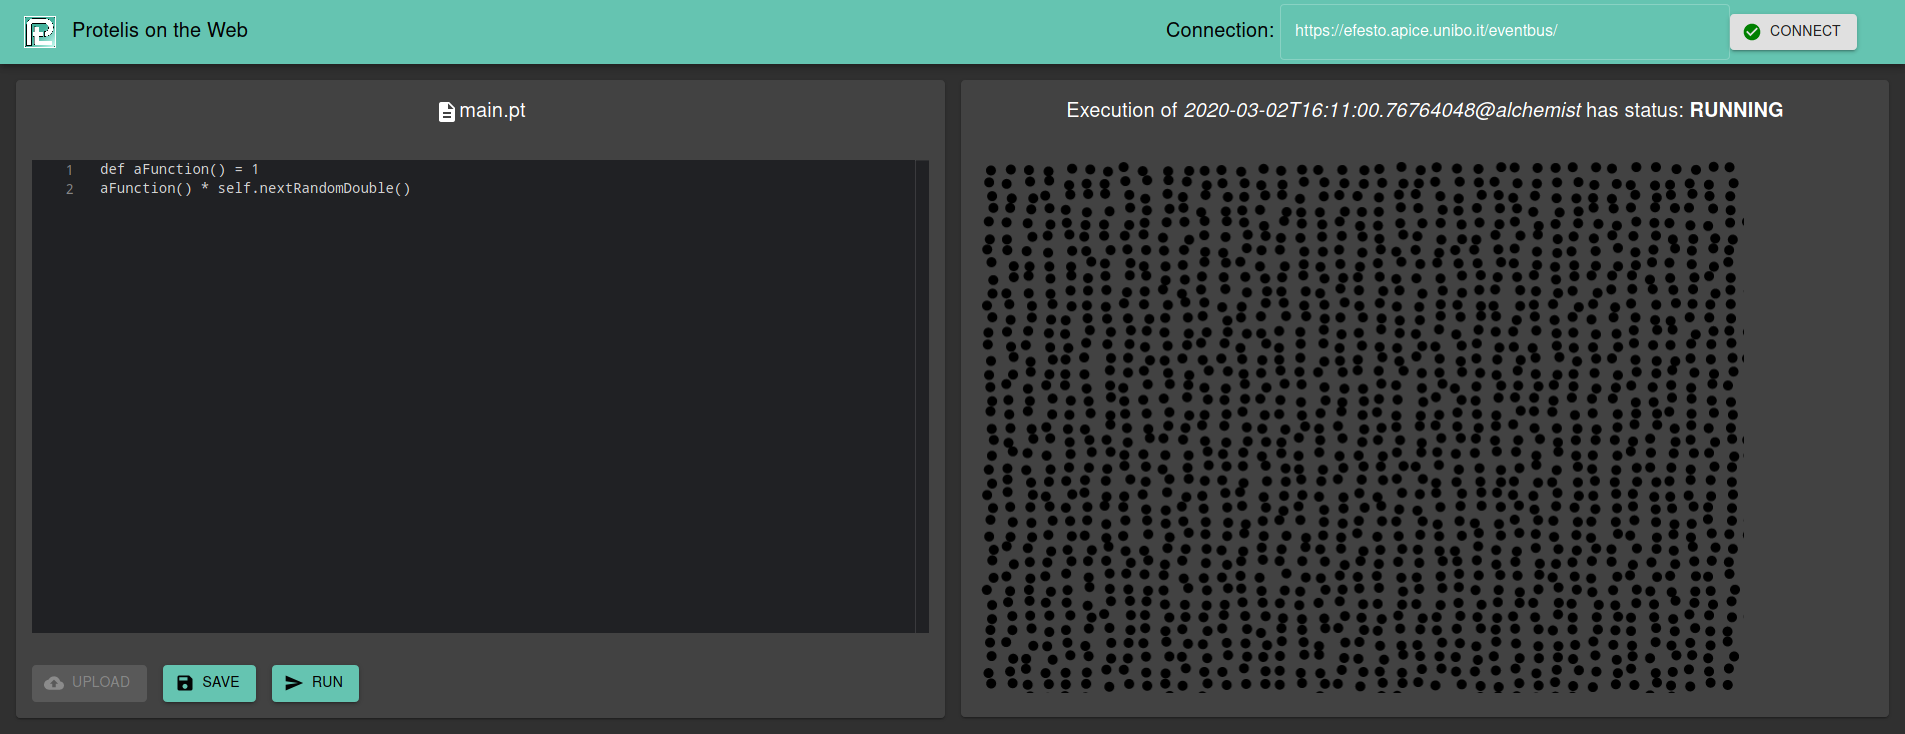
\includegraphics[width=\textwidth]{res/screenshot/Screenshot_2020-03-02 Protelis on the Web(6).png} % ChkTeX 8, ChkTeX 36
      \caption{Screenshot della schermata intera durante l'esecuzione}%
      \label{fig:screenshot:all}
    \end{figure}

    La struttura del frontend, visibile in~\Cref{fig:screenshot:all}, è composta da tre elementi principali:

    \begin{itemize}
      \item
        la \texttt{AppBar} superiore, nella quale è posizionato il selettore con il quale è possibile indicare quale server di backend utilizzare.
      \item
        la \texttt{Card} di sinistra ospita tutti i controlli principali.
        In essa è presente un editor realizzato con l'ausilio della libreria Monaco Editor, realizzata da Microsoft e utilizzata, ad esempio, per Visual Studio Code;
        Essa supporta buona parte dei plugin disponibili per tale IDE e lascia spazio, in futuro, all'integrazione di \emph{language server} dedicati all'autocompletamento.

        Sotto l'editor sono presenti i bottoni dedicati al salvataggio del codice e all'avvio dell'esecuzione.
      \item
        la \texttt{Card} di destra ospita invece principalmente un canvas, realizzato tramite la libreria Konva.
        Essa permette di realizzare canvas performanti modellando ciascuna operazione di disegno come componenti React.

        È risultato dunque semplice delegare le operazioni di disegno al motore di React, attraverso un'operazione di binding dei componenti di Konva con lo stato interno del sistema.
    \end{itemize}

    La gestione dello stato, come deciso in fase di progettazione, è delegata alla libreria Redux;
    in particolare, si è scelto di utilizzare lo strumento ufficiale \texttt{redux-toolkit}, che permette una configurazione dello store ottimale riducendo il codice \emph{boilerplate}.

    Per memorizzare le informazioni sullo stato del sistema, le due \emph{slice} illustrate alla~\Cref{subsec:state-manage} sono state sufficienti.
    \unsure{Dovrei dire altro?}

    Per quanto riguarda la gestione del protocollo di comunicazione, invece, è stato necessario realizzare un \emph{middleware} che incapsulasse la comunicazione.

    In Redux, un \emph{middleware} è una funzione che si frappone tra il \emph{dispatcher} e il \emph{reducer} e permette l'elaborazione dell'azione prima che essa venga gestita.
    Attraverso un middleware, è possibile definire comportamenti asincroni senza rallentare la gestione delle permutazioni sullo stato:
    esso può infatti ``catturare'' azioni provenienti da componenti di controllo nella pagina richiedenti operazioni bloccanti e, una volta che il processo asincrono è terminato, generare un'azione per aggiornare lo stato.

    Sono stati sviluppati numerosi middleware per la gestione delle websocket, ma non ne sono stati trovati in grado di supportare SockJS\@.
    Si è deciso dunque di definirne uno che nascondesse l'intera procedura di connessione, gestendo le azioni che permettono la connessione, la disconnessione e l'invio di messaggi e aggiornando lo stato quando necessario.

    Poiché l'intera logica di connessione è nascosta, in futuro sarà possibile, se necessario, sostituire il protocollo di comunicazione senza che altre modifiche siano necessarie al sistema.

  \section{Dettagli implementativi: Backend}

    Come progettato nella~\Cref{sec:arch:server}, il server è stato realizzato con due verticle di Vert.x che modellano la logica applicativa e uno dedicato all'avvio del sistema.
    Tali verticle comunicano tra loro e con l'esterno tramite EventBus.

    L'EventBus viene esposto verso l'esterno tramite la libreria ufficiale di Vert.x per la realizzazione di bridge con SockJS\@.
    In particolare, la classe \texttt{BridgeVerticle} si occupa di costruire un router HTTP e HTTPS sul quale viene montato il bridge.

    La gestione della simulazione avviene, come detto, appoggiandosi ad Alchemist (il diagramma UML in~\Cref{fig:server:uml} mostra le principali classi coinvolte).

    \begin{figure}[htbp]
      \centering
      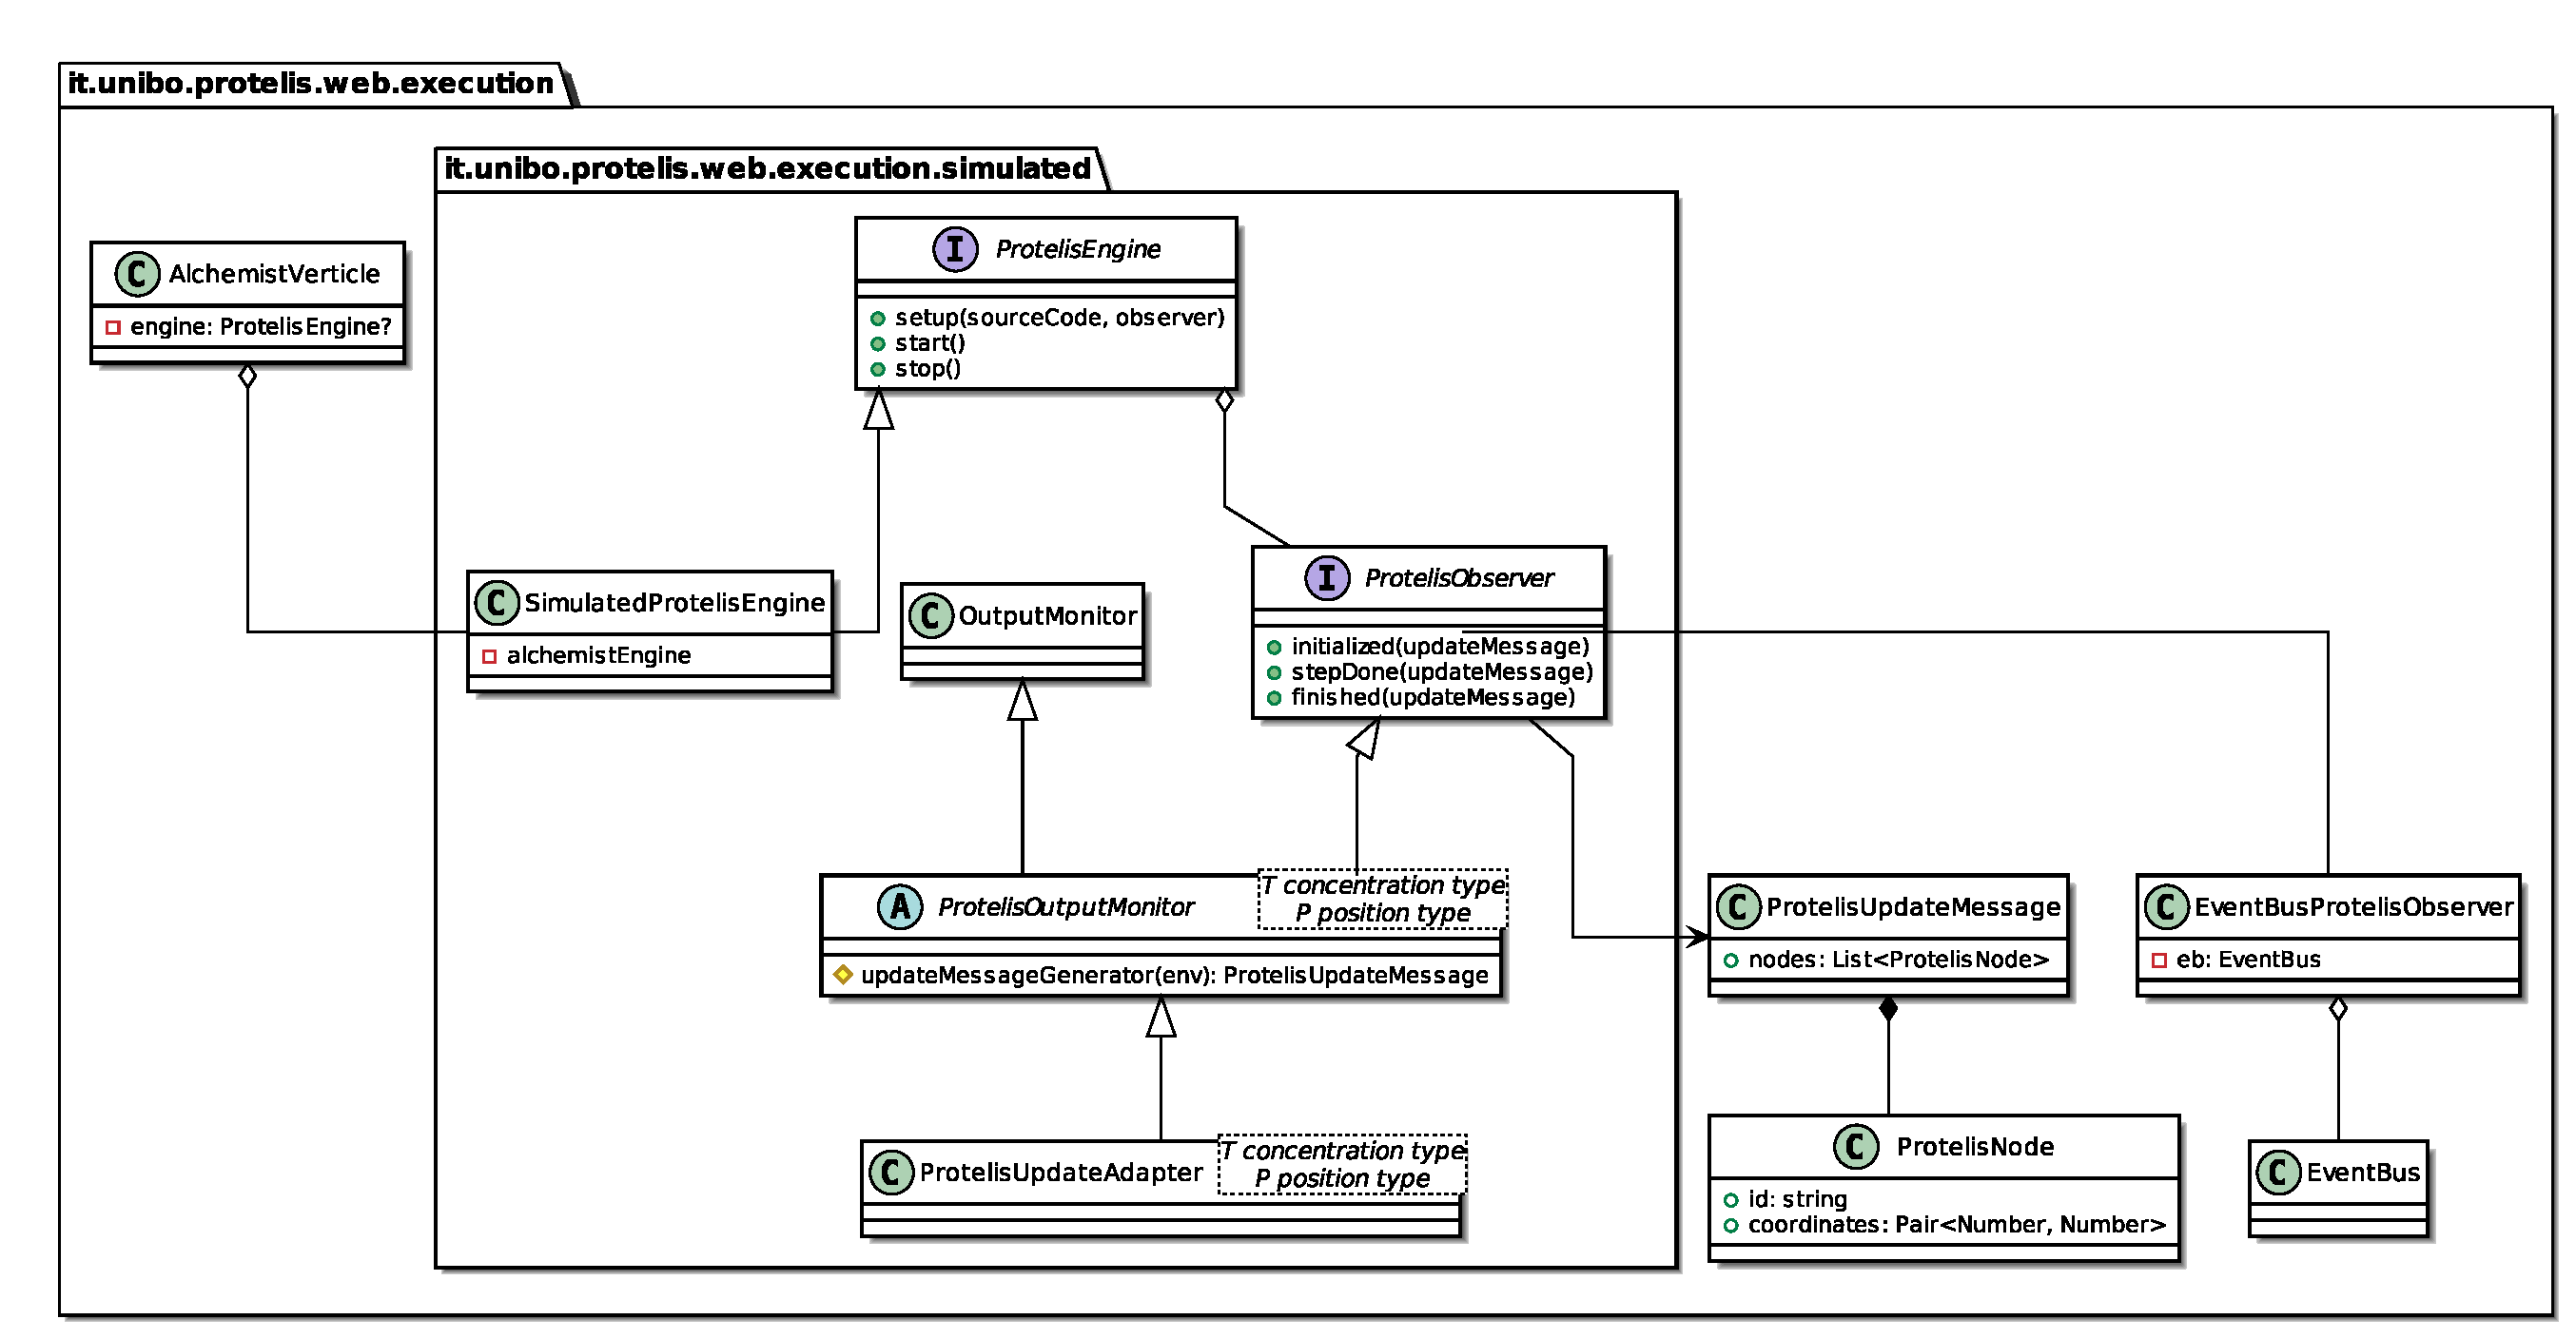
\includegraphics[width=\textwidth]{res/uml/engine-simple.eps}
      \caption{Rappresentazione UML delle classi coinvolte nella simulazione}%
      \label{fig:server:uml}
    \end{figure}

    Come è possibile vedere, Alchemist non viene utilizzato direttamente, bensì incapsulato all'interno di un \texttt{SimulatedProtelisEngine}.
    Tale classe implementa l'interfaccia \texttt{ProtelisEngine}, che astrae il concetto di esecutore per codice Protelis;
    in questo modo, il sistema non è vincolato all'implementazione simulata, né essa è legata strettamente ad Alchemist.

    Anche l'astrazione di Alchemist per l'osservazione del motore di esecuzione è stata incapsulata, definendo una classe di \emph{boundary}, \texttt{ProtelisOutputMonitor}, che agisce da adattatore.


  \part{Conclusioni}\label{part:conclusion}
    \chapter{Valutazione dei risultati}\label{ch:evaluation}

  \section{Qualità del codice e unit testing}
    Durante lo sviluppo, si è cercato di prestare particolare attenzione alla qualità del codice prodotto.

    Si è ritenuto fondamentale, innanzitutto, per favorire la consistenza dello stile, che il codice fosse conforme a uno stile di programmazione riconosciuto.
    Come detto nella~\Cref{subec:quality}, sono stati utilizzati diversi \emph{linter} (ESLint e ktlint)
    per imporre lo stile Airbnb per TypeScript e lo stile ufficiale per Kotlin in tutta la codebase.
    Questo ha permesso di evitare bug comuni riconoscibili attraverso analisi statica
    e potenzialmente permette di rendere il codice, che è pubblico e open-source, maggiormente comprensibile per chi vorrà estenderlo in futuro.

    Inoltre, per garantire il corretto funzionamento delle componenti più cruciali, sono stati creati degli specifici unit test in grado di coprire il codice per quanto possibile.
    L'esecuzione dei test viene effettuata automaticamente da Travis CI su diverse piattaforma ad ogni operazione di push.

    Per quanto riguarda il backend è stato utilizzato JUnit 5 con l'ausilio delle estensioni di Vert.x.
    I report sulla copertura vengono raccolti tramite JaCoCo.

    \unsure[inline]{Quali dettagli dovrei fornire dei test del backend?}

    Anche il frontend è stato testato tramite unit testing.
    In particolare, si è utilizzato la suite Jest per l'esecuzione dei test e la raccolta dei dati di copertura.

    \unsure[inline]{Quali dettagli dovrei fornire dei test del frontend?}

  \section{Valutazione dell'interfaccia}
    Per quanto riguarda la valutazione del client, è stata presa in considerazione principalmente l'esperienza finale dal punto di vista dell'utente web.
    Per avere una misura quantitativa di quanto l'applicazione web si presenti adeguata, si è deciso di utilizzare lo strumento Lighthouse messo a disposizione da Google.

    \emph{Lighthouse} è uno strumento automatizzato open-source, fornito inizialmente con la suite di strumenti \emph{Chrome DevTools}, che permette l'\emph{auditing} di pagine web secondo gli standard premiati dal motore di ricerca di Google.
    Esso verifica le prestazioni di caricamento e navigazione, l'accessibilità, la SEO (\emph{\emph{S}earch \emph{E}ngine \emph{O}ptimization}), e in generale le buone pratiche di programmazione.
    Supporta inoltre controlli aggiuntivi per le PWA (\emph{\emph{P}rogressive \emph{W}eb \emph{A}pp}) se abilitati.

    \begin{figure}
      \centering
      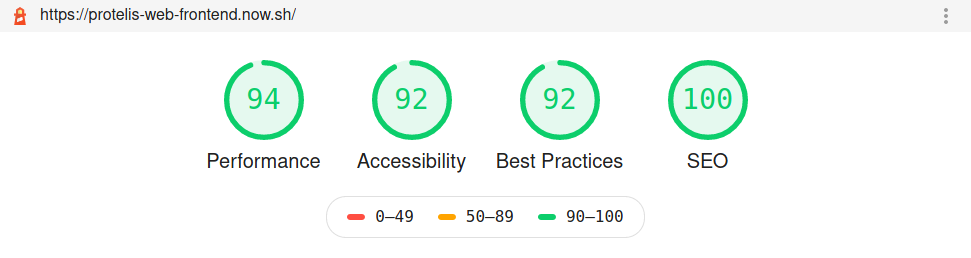
\includegraphics[width=\textwidth]{res/tests/Screenshot_2020-03-04 Lighthouse Report Viewer.png}%
      \caption{Punteggio ottenuto con Google Lighthouse}%
      \label{fig:lighthouse}
    \end{figure}

    Come è possibile vedere in~\Cref{fig:lighthouse}, l'applicazione web ha ottenuto un buon punteggio generale.

    I punteggi di accessibilità e \emph{best practices} sono strettamente legati dalle librerie impiegate, sia in positivo che in negativo:
    il valore elevato deriva da ottimizzazioni della libreria stessa sui componenti che fornisce, cercando di aderire quanto possibile agli standard più moderni;
    le criticità che non portano al 100\% sono legate a limiti difficilmente aggirabili se non configurazioni complesse e fuori tema rispetto all'obiettivo di questa tesi.

    Il punteggio massimo per la SEO, ottenuto ottimizzando la configurazione base generata da React, garantisce, secondo quanto dichiarato da Google, una migliore compatibilità con i motori di ricerca e dunque un ranking migliore.

    Le performance, sulle quali si ha avuto maggiore controllo durante l'implementazione, sono buone, con tempi di primo disegno inferiori al secondo e un ritardo prima di avere possibilità di interazione intorno a \SI{1.6}{\second}.
    A pesare sul punteggio vi è l'assenza di gestione della cache delle richieste, funzionalità non ritenuta importante in questo progetto.

    Volendo ottimizzare ulteriormente, si potrebbe aggiungere il supporto allo standard PWA, secondo le \emph{best practices} documentate da Google.

  % \section{Performance}
  %   % TODO
  %   \unsure[inline]{Come valuto i risultati? Misure di Performance?}

    \chapter{Lavori futuri}\label{ch:future}

  Il lavoro realizzato per questa tesi si pone come punto di partenza per diverse possibili modifiche.

  In primo luogo, l'implementazione attuale si focalizza sulla \emph{simulazione} di una rete di dispositivi, ma rimane aperto ad altre alternative.
  Ad esempio, è possibile rimpiazzare Alchemist con un utilizzo di più basso livello degli strumenti offerti dal framework di Protelis, andando a definire una differente implementazione dell'interfaccia \texttt{ProtelisEngine}.
  \improvement{Dovrei inserire qualche dettaglio progettuale aggiuntivo?}
  Oppure, sarebbe possibile allacciare al sistema una rete fisica di dispositivi, utilizzando un verticle come \emph{bridge} tra il sistema e la rete.

  Per come è stata progettata l'architettura di questo prototipo, ciascuno di questi aggiornamenti non richiederebbe pesanti modifiche:
  in molti casi, la semplice aggiunta di un verticle sarebbe sufficiente.

  Un altro aspetto su cui sarebbe interessante porre l'attenzione in futuro sarebbe la scalabilità:
  come detto nella~\Cref{sec:arch:server}, il prototipo è stato realizzato con un architettura considerabile monolitica, ma il framework offre molte libertà.
  Vert.x permette infatti l'esecuzione di singoli verticle (ed eventuali dipendenze) in modo indipendente, realizzando, di fatto, dei microservizi.
  Esso offre inoltre il supporto a diversi strumenti per l'integrazione con tecnologie per il \emph{service discovery}, per lo scambio di messaggi e per il bilanciamento del carico.\improvement{Dovrei citare più nel dettaglio tali tecnologie?}

  Una soluzione interessante di deploy potrebbe vedere, ad esempio, diversi verticle pacchettizzati come container Docker ed eseguiti in una piattaforma basata su Kubernetes o OpenShift,
  delegando a quest'ultimo livello PaaS il deploy di repliche per l'incremento delle performance on-demand.

  Spostando l'attenzione sul client, potrebbe essere utile aumentare le possibilità di interazione con l'esecuzione.
  Potrebbe, ad esempio, risultare utile la possibilità di interagire con i nodi rappresentati, spostandoli e vedendo così l'esecuzione adattarsi alla perturbazione.
  Funzionalità di questo tipo possono essere inserite in modo abbastanza semplice tramite la realizzazione di eventi specifici, generati dai componenti React e inoltrati tramite SockJS verso il server.

  Infine, un ultimo approccio di miglioramento potrebbe coinvolgere il cambio di parte delle tecnologie impiegate.
  Per la realizzazione di questo prototipo si è ritenuto l'uso di TypeScript ottimale per le ragioni espresse nelle \Cref{subsec:ts,subsec:kotlinjs,subsub:ts},
  ma, potenzialmente, Kotlin potrebbe essere una soluzione molto interessante una volta che avrà raggiunto una stabilità accettabile per il target JS\@.
  Tale migrazione permettere una condivisione più efficiente delle componenti di modello condivise e potenzialmente delle dipendenze.
  Inoltre, collaborando con il team che mantiene il progetto Protelis, sarebbe potenzialmente possibile realizzare un'implementazione locale al client dell'interprete.
  In questo modo, il ruolo del server potrebbe diventare non più necessario per piccoli progetti a scopo educativo come quelli a cui questo progetto ha fatto riferimento fin dall'inizio.

    \chapter{Considerazioni finali}\label{ch:considerations}
  L'obiettivo della tesi era quello di progettare un sistema che permettesse, senza particolari configurazioni,
  di scrivere codice aggregato ed eseguirlo su una rete di esempio.
  Esso doveva essere facilmente accessibile e immediatamente utilizzabile, dunque si è scelto di indirizzarsi verso tecnologie web.

  Per la realizzazione del prototipo, ci si è focalizzati su un solo linguaggio di programmazione aggregata: Protelis.
  Inoltre, per motivi di realizzabilità concreta, si è deciso di simulare la rete di dispositivi su cui eseguire il codice,
  anziché utilizzarne una fisica.

  La realizzazione del sistema nel suo complesso ha comportato la progettazione di due applicazioni su differenti piattaforme e con diverse tecnologie e linguaggi:
  la componente server è stata realizzata avvalendosi del framework Vert.x nel linguaggio Kotlin,
  mentre l'interfaccia web è stata implementata come Single-Page Application avvalendosi di React in TypeScript.

  Per la soddisfazione dei requisiti è stato dunque richiesto uno studio approfondito, anche a causa della profonda diversità di questi due sistemi.
  La decisione di appoggiarsi a soluzioni per la programmazione web moderne è stata però fondamentale per ottenere un sistema davvero di uso immediato come richiesto.

  Nonostante il sistema realizzato sia correttamente funzionante e soddisfi i requisiti, esso è da considerarsi un prototipo e, soprattutto con l'impiego di piattaforme economiche come quelle fornite con il piano \emph{Free} di Heroku, non sarebbe in grado di reggere il carico di un elevato numero di utenti.
  L'attenzione dedicata in fase di progettazione, però, lascia aperte molte strade per l'implementazione in modo semplice di soluzioni maggiormente adatte a casi d'uso complessi.

  Si ritiene dunque che il lavoro svolto abbia raggiunto gli obiettivi prefissati, diventando un'occasione formativa notevole e portando alla realizzazione di un sistema potenzialmente molto utile per la divulgazione della programmazione aggregata.


  \addpart*{\appendixname}

% % \renewcommand{\thesection}{\Alph{section}}
% % \renewcommand{\thesubsection}{A.\arabic{subsection}}

% % \addcontentsline{toc}{section}{\appendixname}
% % \addchap{\appendixname}
% % \chapter*[]{\appendixname}

\appendix
\begin{appendices}

  % \section{Dockerfile del server}\label{app:docker}
  \chapter{Dockerfile del server}\label{app:docker}
  % \addchap*{Dockerfile del server}\label{app:docker}

    Di seguito è riportato il codice del Dockerfile che permette il deploy del server come container Docker.
    L'immagine costruita durante lo sviluppo è anche disponibile su Docker Hub con il nome \texttt{niccomlt/protelis-web}.

    \inputminted{dockerfile}{res/code/Dockerfile}

  % \section{YAML di configurazione per Alchemist}
  \chapter{YAML di configurazione per Alchemist}\label{app:yaml}
  % \addchap*{YAML di configurazione per Alchemist}

    Di seguito è riportata la configurazione in formato YAML che permette ad Alchemist di costruire la rete simulata sulla quale viene eseguito il codice.

    \inputminted{yaml}{res/code/simulation.yml}

\end{appendices}


  \backmatter{}
  \addchap*{Ringraziamenti}


Sono ormai giunto al termine di questo mio percorso universitario
e per questo devo ringraziare di cuore tutte le persone che mi hanno accompagnato lungo questi cinque anni.

Ringrazio i miei genitori, che mi hanno materialmente permesso di compiere questo percorso e mi hanno supportato nei momenti di difficoltà.
Ringrazio anche gli altri miei familiari che mi hanno sostenuto negli anni.

Ringrazio poi tutti gli amici che mi sono stati vicino in questo percorso:
coloro con cui ho condiviso i progetti ingestibili e le infinite sessioni di studio in biblioteca o al campus,
coloro con cui da sempre condivido serate di spensieratezza,
coloro che ho scoperto o ritrovato con l'università.

Infine ringrazio il professor Mirko Viroli e il professor Danilo Pianini
per la bella opportunità che mi hanno offerto,
per l'aiuto datomi per realizzare questo progetto
e per le competenze che mi hanno permesso di sviluppare.

Grazie a tutti, di cuore.

  % \nocite{7274429,PianiniSASOTutorial2017}
\printbibliography[heading=bibintoc]


\end{document}
